
\documentclass[twoside]{article}


% ------
% Fonts and typesetting settings
\usepackage[sc]{mathpazo}
\usepackage[T1]{fontenc}
\linespread{1.05} % Palatino needs more space between lines
\usepackage{microtype}
\usepackage{textcomp}


% ------
% Page layout
\usepackage[hmarginratio=1:1,top=32mm,columnsep=20pt]{geometry}
\usepackage[font=it]{caption}
\usepackage{multicol, hyperref}
\usepackage{parskip}

% ------
% Lettrines
\usepackage{lettrine}
\usepackage{color}

% ------
% Abstract
\usepackage{abstract}
	\renewcommand{\abstractnamefont}{\normalfont\bfseries}
	\renewcommand{\abstracttextfont}{\normalfont\small\itshape}


% ------
% Titling (section/subsection)
\usepackage{titlesec}
\renewcommand\thesection{\Roman{section}}
\titleformat{\section}[block]{\large\scshape\centering}{\thesection.}{1em}{}


% ------
% Header/footer
\usepackage{fancyhdr}
	\pagestyle{fancy}
	\fancyhead{}
	\fancyfoot{}
	\fancyhead[C]{ $\bullet$ Draft $\bullet$}
	\fancyfoot[RO,LE]{\thepage}

% My Shortcuts 

%useful shortcuts
\def\R{\ensuremath{\mathbb{R}}} %\ensuremath adds math mode, if forgotten
\def\Q{\ensuremath{\mathbb{Q}}}
\def\N{\ensuremath{\mathbb{N}}}
\def\Z{\ensuremath{\mathbb{Z}}}
\def\C{\ensuremath{\mathbb{C}}}

%shorcuts with arguments
\newcommand{\abs}[1]{\left\vert#1\right\vert} %nice absolute values
\newcommand{\bt}[1]{\textbf{#1}} %bold
\newcommand{\eq}[1]{\begin{align*}#1\end{align*}} %aligned equations
\newcommand{\cb}[1]{\centerline{\fbox{#1}}} %centered box
\newcommand{\bp}[1]{\fbox{\parbox{0.8\textwidth}{#1}}} %box paragraph
\newcommand{\norm}[1]{\left\lVert#1\right\rVert} %vector norm
\newcommand{\notimplies}{% does not imply
  \mathrel{{\ooalign{\hidewidth$\not\phantom{=}$\hidewidth\cr$\implies$}}}}
\renewcommand{\eq}[1]{\begin{align*}#1\end{align*}} %aligned equations

%colors
\definecolor{javagreen}{rgb}{0.25,0.5,0.35} %dark green color
\definecolor{lightblue}{rgb}{0.149,0.545,0.824} %solarized blue
\definecolor{sred}{rgb}{0.863, 0.196, 0.184} %solarized red

\newcommand{\blue}[1]{{\leavevmode\color{lightblue}{#1}}} %solarized blue 
\newcommand{\green}[1]{{\leavevmode\color{javagreen}{#1}}} %command for green
\newcommand{\red}[1]{{\leavevmode\color{sred}{#1}}} %solarized red
\newcommand{\gray}[1]{{\leavevmode\color[gray]{0.5}{#1}}} %gray text

%environment
\newcommand{\tab}{\phantom{ssss}}
%----------------

% ------
% Clickable URLs (optional)
\usepackage{hyperref}

% ------
% Maketitle metadata
\title{\vspace{-5mm}%
	\fontsize{24pt}{12pt}\selectfont
	\textbf{What's so Special about Philosophy?} 
	}	
\author{%
\fontsize{14pt}{14pt}\selectfont
	Unraveling Wikipedia's First Link Network \vspace{-2mm}\\
	}
\date{}

%figures
\usepackage{graphicx}
\usepackage{caption}
\usepackage{subcaption}
\usepackage{float}

%text, figure spacing
\raggedbottom

%footnote withou marker
\newcommand\blfootnote[1]{%
  \begingroup
    \renewcommand\thefootnote{}\footnote{#1}%
      \addtocounter{footnote}{-1}%
   \endgroup }
%%%%%%%%%%%%%%%%%%%%%%%%
\begin{document}
\maketitle
\thispagestyle{fancy}
%========================ABSTRACT====================================

\begin{abstract}
\fontsize{12pt}{12pt}
\selectfont

Apples, oranges, and the most obscure Dylan song too---is everything a few clicks from Philosophy? 
Within Wikipedia, the surprising answer is yes: nearly all 
paths lead to Philosophy.
\footnote{
nearly $99.6\%$ of First Link paths, ending inside Wikipedia, lead to the Philosophy article (see traversal funnels discussion for details).}
\footnote{
An analysis performed in 2011 by Mat Kelcey posted on his blog (and a smiliar post by Ilmari Karonen) suggest $94.5\%$ of articles end up at Philosophy.
}
Wikipedia is the largest, most meticulously indexed collection of human knowledge ever amassed. 
\footnote{
cite MIT Tech Review Article: http://www.technologyreview.com/featuredstory/520446/the-decline-of-wikipedia/
}
More than information about a topic though, Wikipedia is a marvelous web of naturally emerging relationships.  
By following the First Link in an article, we connect entries to form a directed network within Wikipedia: Wikipedia's First Link Network. 
Here we study the English edition of Wikipedia's First Link Network for insight into how we relate topics, ideas, people, objects, and events.  


We algorithmically parse all 4.7 million articles to construct a map of Wikipedia's First Link Network. 
In a novel approach to uncover structure, we traverse every possible path through the network, 
measuring the accumulation of First Links, path lengths, basins, cycles, and even particular articles funneling links into the cycles.
We discover many scale-free distributions, find Philosophy at a salient center, and uncover a flow from specific to general with 
basins around fundamental notions such as Community, State, and Science. 
Curiously, we also observe a gravitation towards topical articles including Health Care and Fossil Fuel.
These findings enrich our view of how we connect and structure
an ever growing load of information.

\end{abstract}

\fontsize{11pt}{11pt}
\selectfont

%========================INTRODUCTION====================================
At no point in history has a larger or more meticulously indexed collection of human knowledge existed.
In amassing such an awe-inspiring collection, we formed an equally impressive web. 
Through the efforts of millions of individuals, working independently,
((cite))
we naturally linked topics, inventions, people, objects, places, and events across space and time.
The web we weaved, and continue to weave, is a wealth of information not only about those notable inventions, 
places, figures, and ideas, but also about \textit{relationships} among them.
We study the relationships in this naturally arising web through the hyperlinks connecting one article to another.

We build Wikipedia's First Link Network by following the First Link, not in parenthesis, inside the main body of each article in the English edition of Wikipedia. 
For the directed network to meaningfully reflect how we associate one article to another, we exclude links in parenthesis, 
disregarding pronunciation keys or disambiguations.
We also exclude any links in the side-bar elements, as well as any links to external pages, files, or WikiMedia 
projects outside of Wikipedia (such as Wiktionary).
This procedure corresponds to the original claim in 2008 about the percentage of pages with First Links to 
"Philosophy."\footnote{
https://en.wikipedia.org/wiki/Wikipedia:GettingtoPhilosophy
}
\footnote{
http://xkcd.com/903/
}
\footnote{
https://www.reddit.com/r/pics/comments/gpdhb/trythiswikipediamindfk/
}

The result is a directed network placing every article in a broader web of ideas.


\begin{figure}[H]
\centering
\caption{Wikipedia Train}
    \begin{subfigure}[b]{0.8\textwidth}
        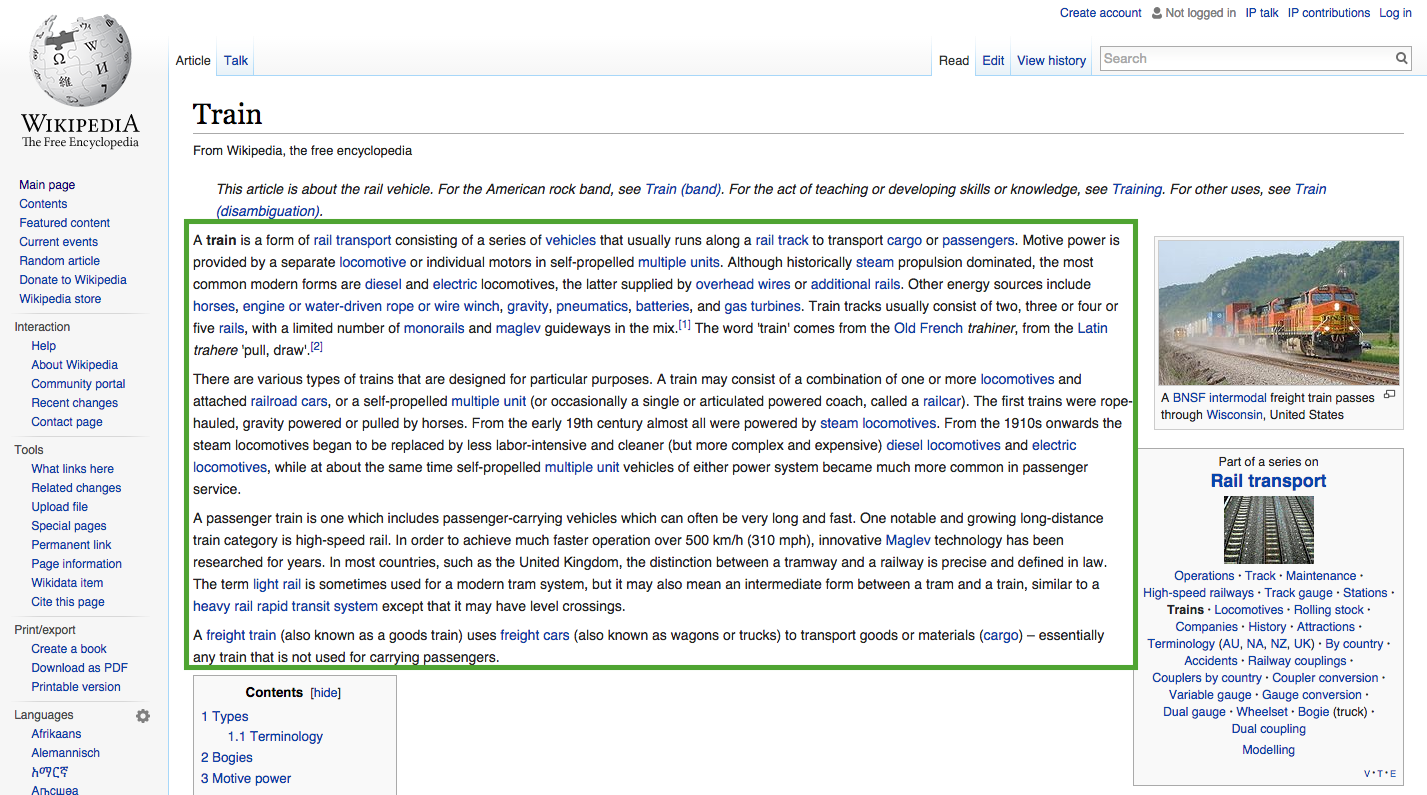
\includegraphics[width=\textwidth]{graphics/wiki_train.png}    
    \end{subfigure}
\end{figure}

%===========================Data_and_Parsing================================
\section{Constructing the First Link Network}

To map Wikipedia's First Link Network, we use the freely-available XML dump of the English edition of Wikipedia. 
Rather than rely on a sample of articles from which to generalize, we opted to process the entirety of Wikipedia, 
eliminating any statistical error due to sampling.
We analyze the snapshot provided on November 2014, representing the state of Wikipedia at the time.
The November raw dump consists of 11 million articles: 4.7 million unique articles along with redirects
and disambiguations.
Knowing Wikipedia is an ever-evolving project with 10 edits every second and 750 new articles per day on average
((cite)), our aim is to characterize the dynamics of the First Link Network, not record a particular link between one
article and another.

Wikipedia renders and stores articles in MediaWiki markup, a markup langauge with syntax and keywords to format and mark elements in a page. Along with special syntax for links, MediaWiki markup includes templates for audio files, images, and side-bar
information.
While a human can accurately identify the First Link, to map the entire First Link Network of 11 million articles, we programmatically untangled the body text from side-bar, header box, and invalid link elements.

While some libraries exist for MediaWiki Markup, we opted to develop our own algorithm for parsing the First Link in the XML version of each article.\footnote{
Approaches using existing libraries led to several bugs 
including trouble with nested links, nested parenthesis, unclosed tags, escape characters 
as well as compatibility with other libraries used to parse the XML.}
Our parsing algorithm aimed to: 
1) accurately identify the First Link among other page elements
2) efficiently do so, without the need for several passes through the data.
To process an article with one pass, we developed a hierarchical system of flags:

\begin{figure}[H]
\centering
\caption{parsing algorithm of Wikipedia's XML dump}
    \begin{subfigure}[b]{0.5\textwidth}
        \includegraphics[width=\textwidth]{graphics/flags.pdf}    
        \caption{ The highest flag in the hierarchy indicates a Wikimedia template used to mark an element in the side bar, display an image, link to an external file, or another Wikimedia project outside of Wikipeida. Next, to catch any remaining elements outside the main body we have a second flag for <ref>, <div> elements. Finally, we catch parenthesis to ensure we do not capture a link to a pronunciation key.}
    \end{subfigure}

\end{figure}

The algorithm loops in three-character chunks to account for potentially nested elements, 
shifting by one character steps through the article markup.
If any markup triggers for a flag are detected, a flag is raised. 
Once a flag is raised, we stop processing and proceed to the next character
until the flag's closing markup.
A First Link is identified only if Flags 1, 2, and 3 are all off.
In this case, the entire link is retrieved. 
We then confirm the link is valid by filtering for MediaWiki keywords indicating external page or other projects
as well as common file extensions for 
((cite))
images, audio files, and the like.
The First Link of an article is then the earliest valid link with unraised flags.

To process the entirety of Wikipedia, we distributed the parsing and processing of the XML dump
across 112 cores of the UVM supercomputer cluster
((cite))
We then joined the results to form a hash table containing every Wikipedia article and its corresponding
First Link. The resulting network map is the basis of our analysis.


%========================Traversing the Network====================================
\section{Traversing the Network}

To understand the structure of Wikipedia's First Link Network, we
aimed to characterize the dynamics of the flow from one article to another. 
Do links tend towards a particular article, group of articles, or various groups of articles? 
What is the flow of links through a typical article?
What types of cycle (loop) structures exist in the network?
What are typical paths from one article to loop or an invalid link? 
Are there exceptionally long or short paths? 
Are there articles funneling the flow of links towards a particular path?
In answering these questions about the directed network, we aimed to characterize 
how so many independent articles relate to each other.

The n-degree, or number of links directly pointing to a particular article,
while a natural measure, fails to fully capture the dynamics needed to answer these questions.
The n-degree measures only the particular set of links to a particular article, 
rather than the richer dynamics of how the links flow through the network: 
where articles tend, what the typical and atypical 
paths through the network are, which articles funnel relatively more links and so on. 

Consequently, to capture the dynamics of how the First Links flow, we actually traverse every possible path through the network. 
We developed three metrics to uncover structure: traversal visits, traversal funnels, and path length. Each metric captures one essence of how the links flow. Traversal visits gauge the accumulation of links; traversal funnels gauge the influence on link path; path length measures the number of First Links to a repeated or invalid link. 


The algorithm for traversing the network begins by selecting any article. We then proceed to the next article by following the First Link---recalling a First Link is a link in the main body of the article leading to another Wikipedia article. We repeat until the First Link is invalid or repeated to form a path. The collection of articles is path-connected conveying a flow of concepts from one article to another. 
The method is order agnostic with respect to which articles are selected first.
As long as each article is selected eventually, the resulting metrics are equivalent.

\begin{figure}[H]
\centering
    \caption{traversal visit algorithm on a sample network}
\begin{subfigure}[b]{\textwidth}
    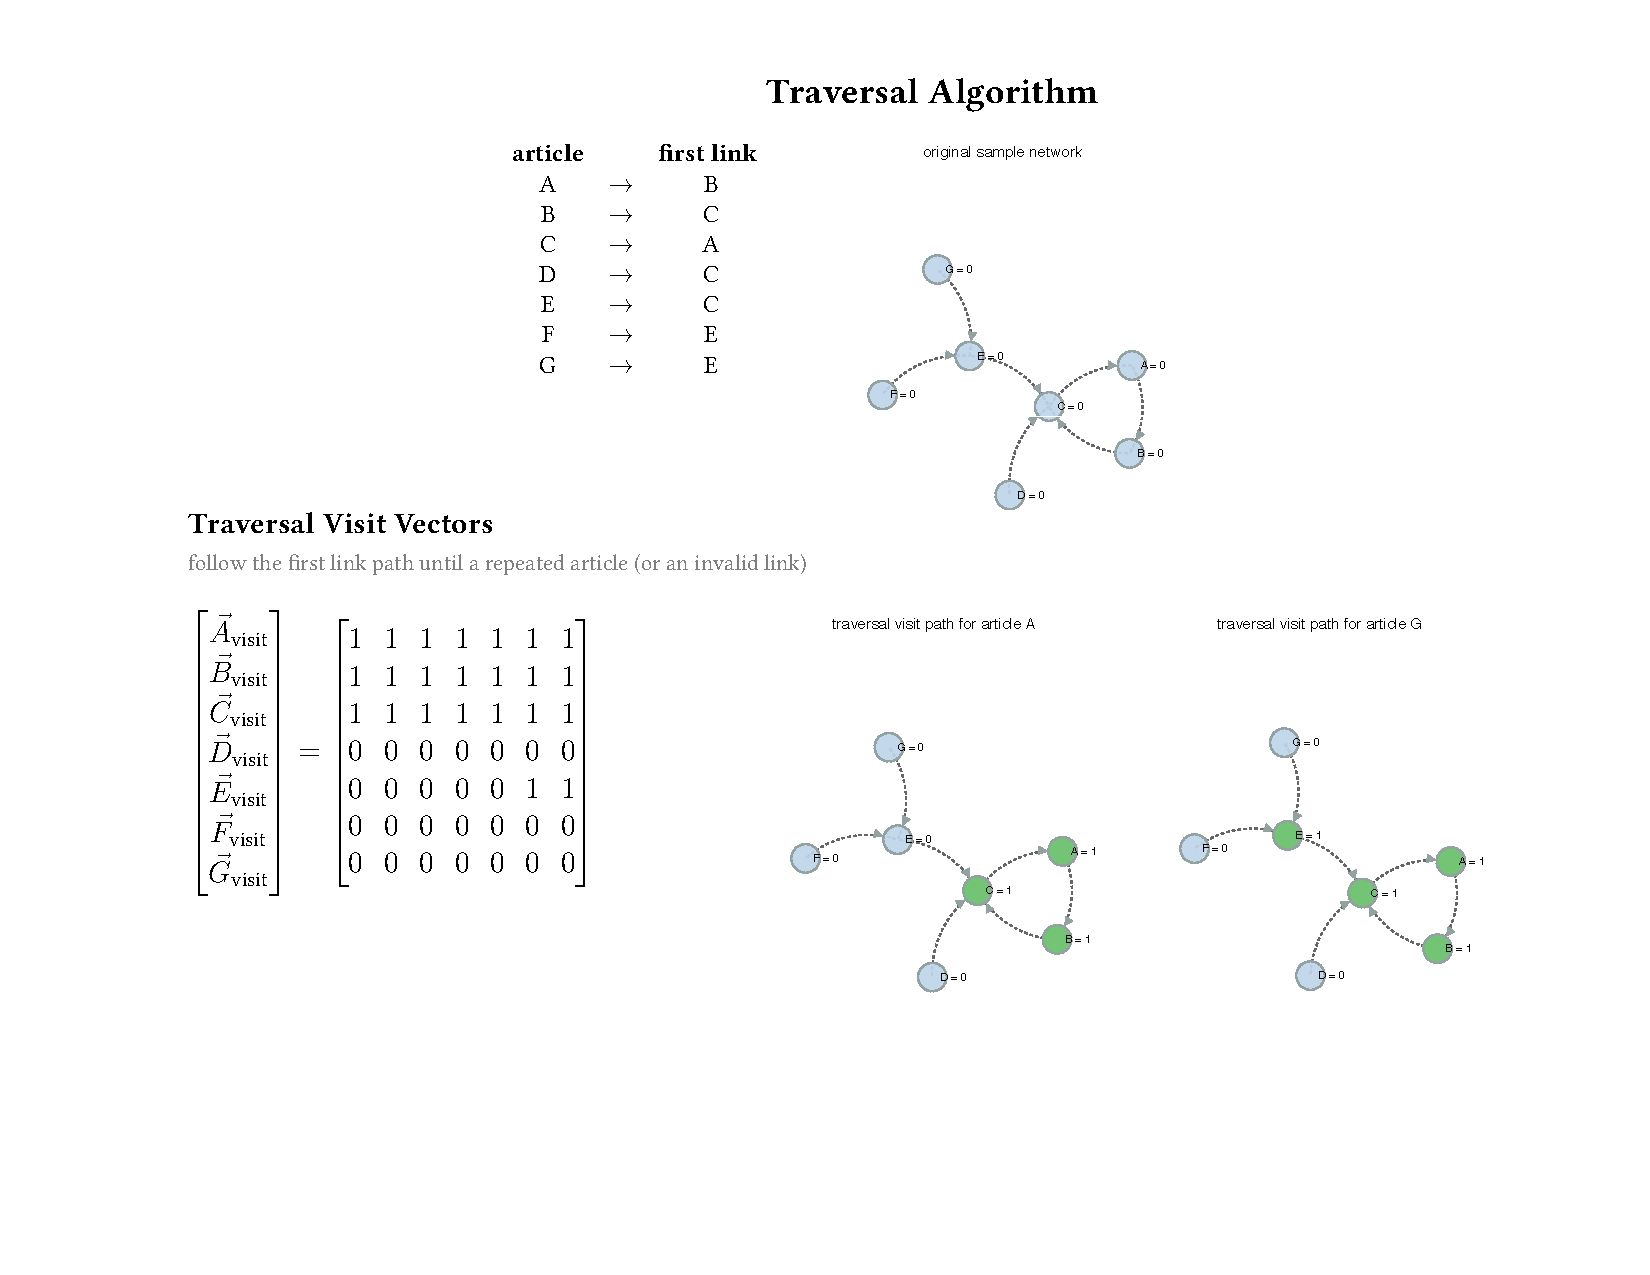
\includegraphics[width=\textwidth]{graphics/traversal_visit_algo_figure.pdf}
    \caption{The traversal visit vectors are an adjacency matrix for the paths through the network: the first column is indicates the path formed starting with article A. The number of traversal visits for article A is then the number of paths containing A or the sum of the first row in our matrix.}
\end{subfigure}
\end{figure}

The first metric, traversal visits, gauges where the flow of first accumulates by associating a count to each article. Every path through the article increments the associated count by 1. We can construct a vector to represent the articles incremented on a particular path, combining these vectors to form a matrix. The total accumulated counts for a given article is then simply the sum of the row in our matrix corresponding to the article of interest. Node A in our example has 7 traversal visits, since every path includes article A. Whereas, node E only has two traversal visits since only two paths contain article E for example.
What we have then is a metric signaling which article contains a larger accumulation of first links.


While traversal visits measure accumulation, we cannot gauge whether a particular article exerts a greater influence on flow of the first link paths. To distinguish between an article that simply happened to fall within a cycle from an article actually funneling the flow of first links, we developed a second metric called traversal funnels. We traverse the network in the same manner, but end our paths once we enter a cycle. We again increment the associated count of each article by one if the path up to a cycle contains the article. We call the accumulated count the number of traversal funnels. By measuring traversal funnels, we quantify
which articles funnel more link paths in a particular direction or cycle.

\begin{figure}[H]
\centering
    \caption{traversal funnel algorithm on a sample network}
\begin{subfigure}[b]{\textwidth}
    \includegraphics[width=\textwidth]{graphics/traversal_funnel_algo_figure.pdf}
    \caption{The algorithm for traversal funnels is identical to the previous algorithm for traversal visits with one alteration: the path ends at the start of a cycle to distinguish articles directing a path into a cycle from articles that simply happen to be in a highly traversed path. We can construct similar vectors by considering each path through the network, measuring traversal funnels for a particular article as the sum of the entries in its corresponding row.}
\end{subfigure}
\end{figure}

Finally, we track the number of links until a repeated article or invalid link, to find the typical path length within the network.
By recording the history of articles we traversed, we are also able to uncover several other network charactersitics including basins, defined as a collection of path-connected articles ranked by traversal visits, and cycles of various lengths.
The three metrics: traversal visits, traversals funnels, and path length, along with our path history
yield a powerful arsenal of information with which to study the network. 


%========================Results====================================
\section{Discoveries}

We followed every possible path through the network, taking 232 million steps along the way to measure the accumulated number of traversal visits.

\subsection{Traversal Visits}

As a distribution, the number traversal visits per article appears scale-free. The majority of articles have fewer than 30 traversal visits, while few 
have 5 order of magnitude more traversal visits. 
Specifically, $99.76\%$ of articles have fewer than $100$ traversal visits; nearly $80\%$ have none. 
Meanwhile, the highest ranking 30 articles have an extremely disproportionate number of traversal visits.

\begin{figure}[H]
\centering
    \caption{distribution of traversal visits}
        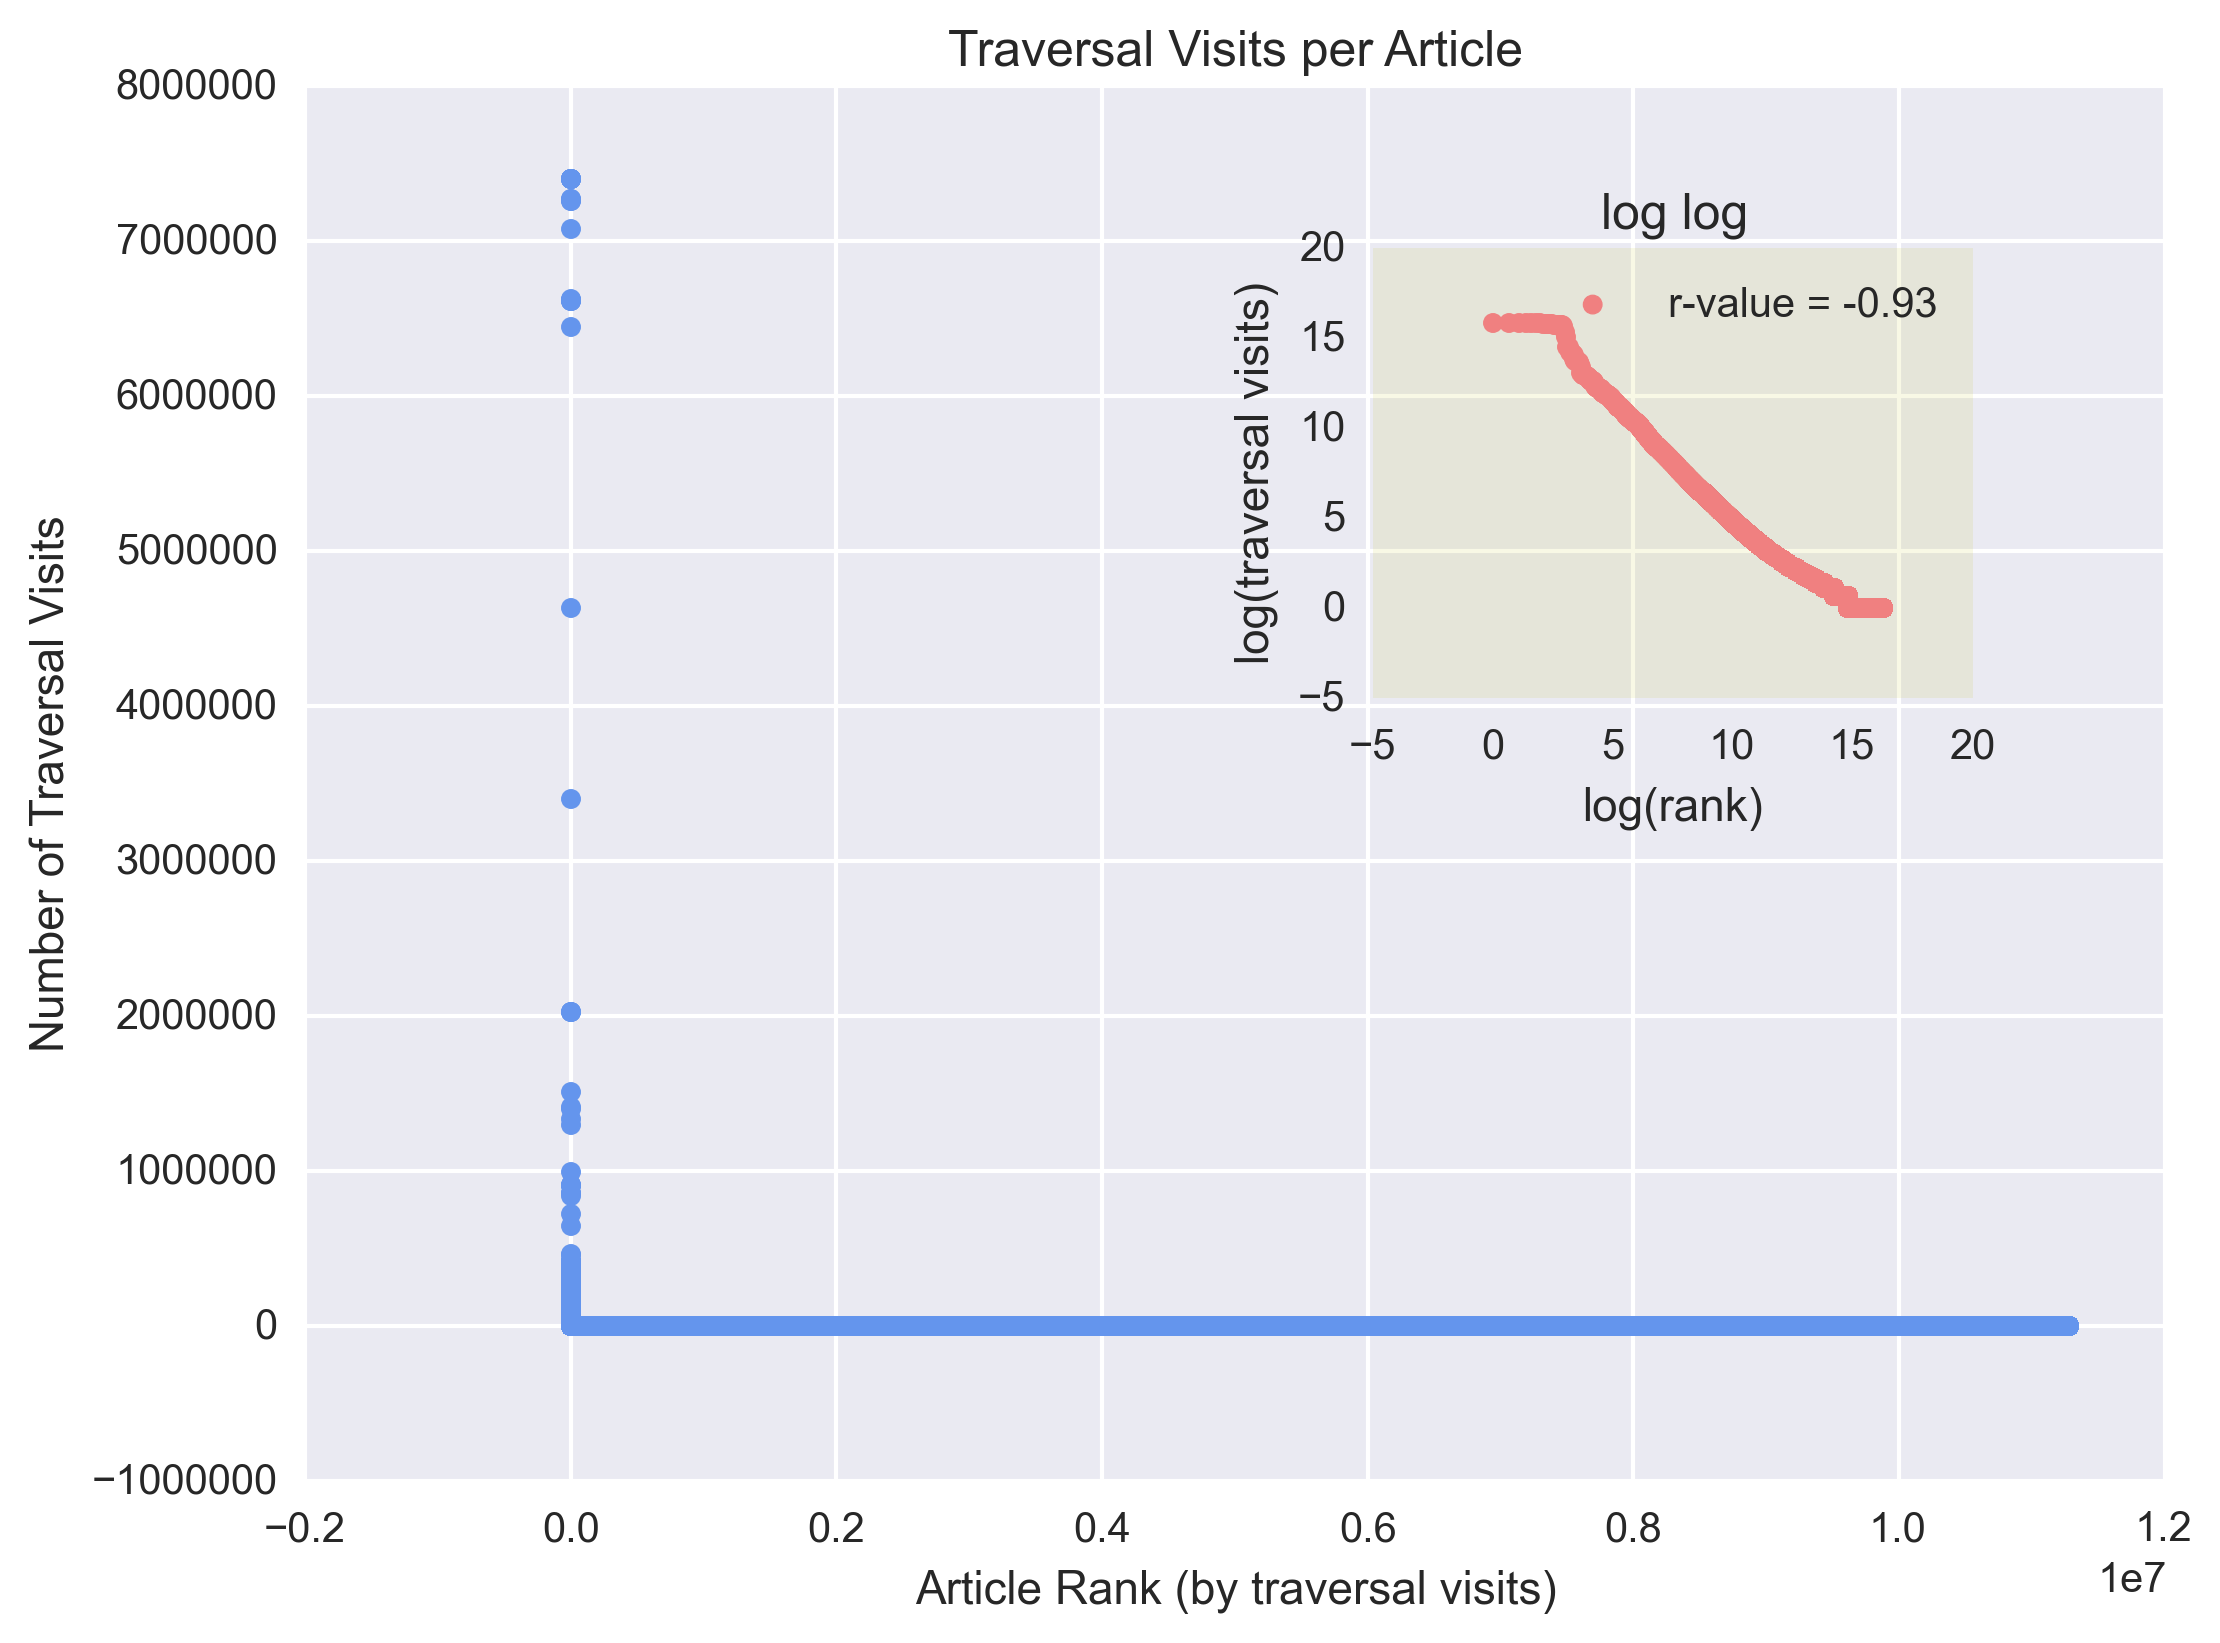
\includegraphics[width=\textwidth]{graphics/traversals_per_article.png}
\end{figure}

To more accurately gauge the distribution, we constructed a log-log plot of the entire dataset: log(traversal visits) against log(rank). We observe a fairly linear fit, as is characteristic of scale-free networks, with an r-value of -.93. A handful of the highest ranking articles contain a disproportionate number of traversal visits, while most have none. The skew in the distribution is not terribly surprising when considering the heuristic of how the links flow: from specific to general. 

\begin{figure}[H]
\centering
\caption{traversal visit distribution of highest ranking articles}
\begin{subfigure}{.5\textwidth}
  \centering
  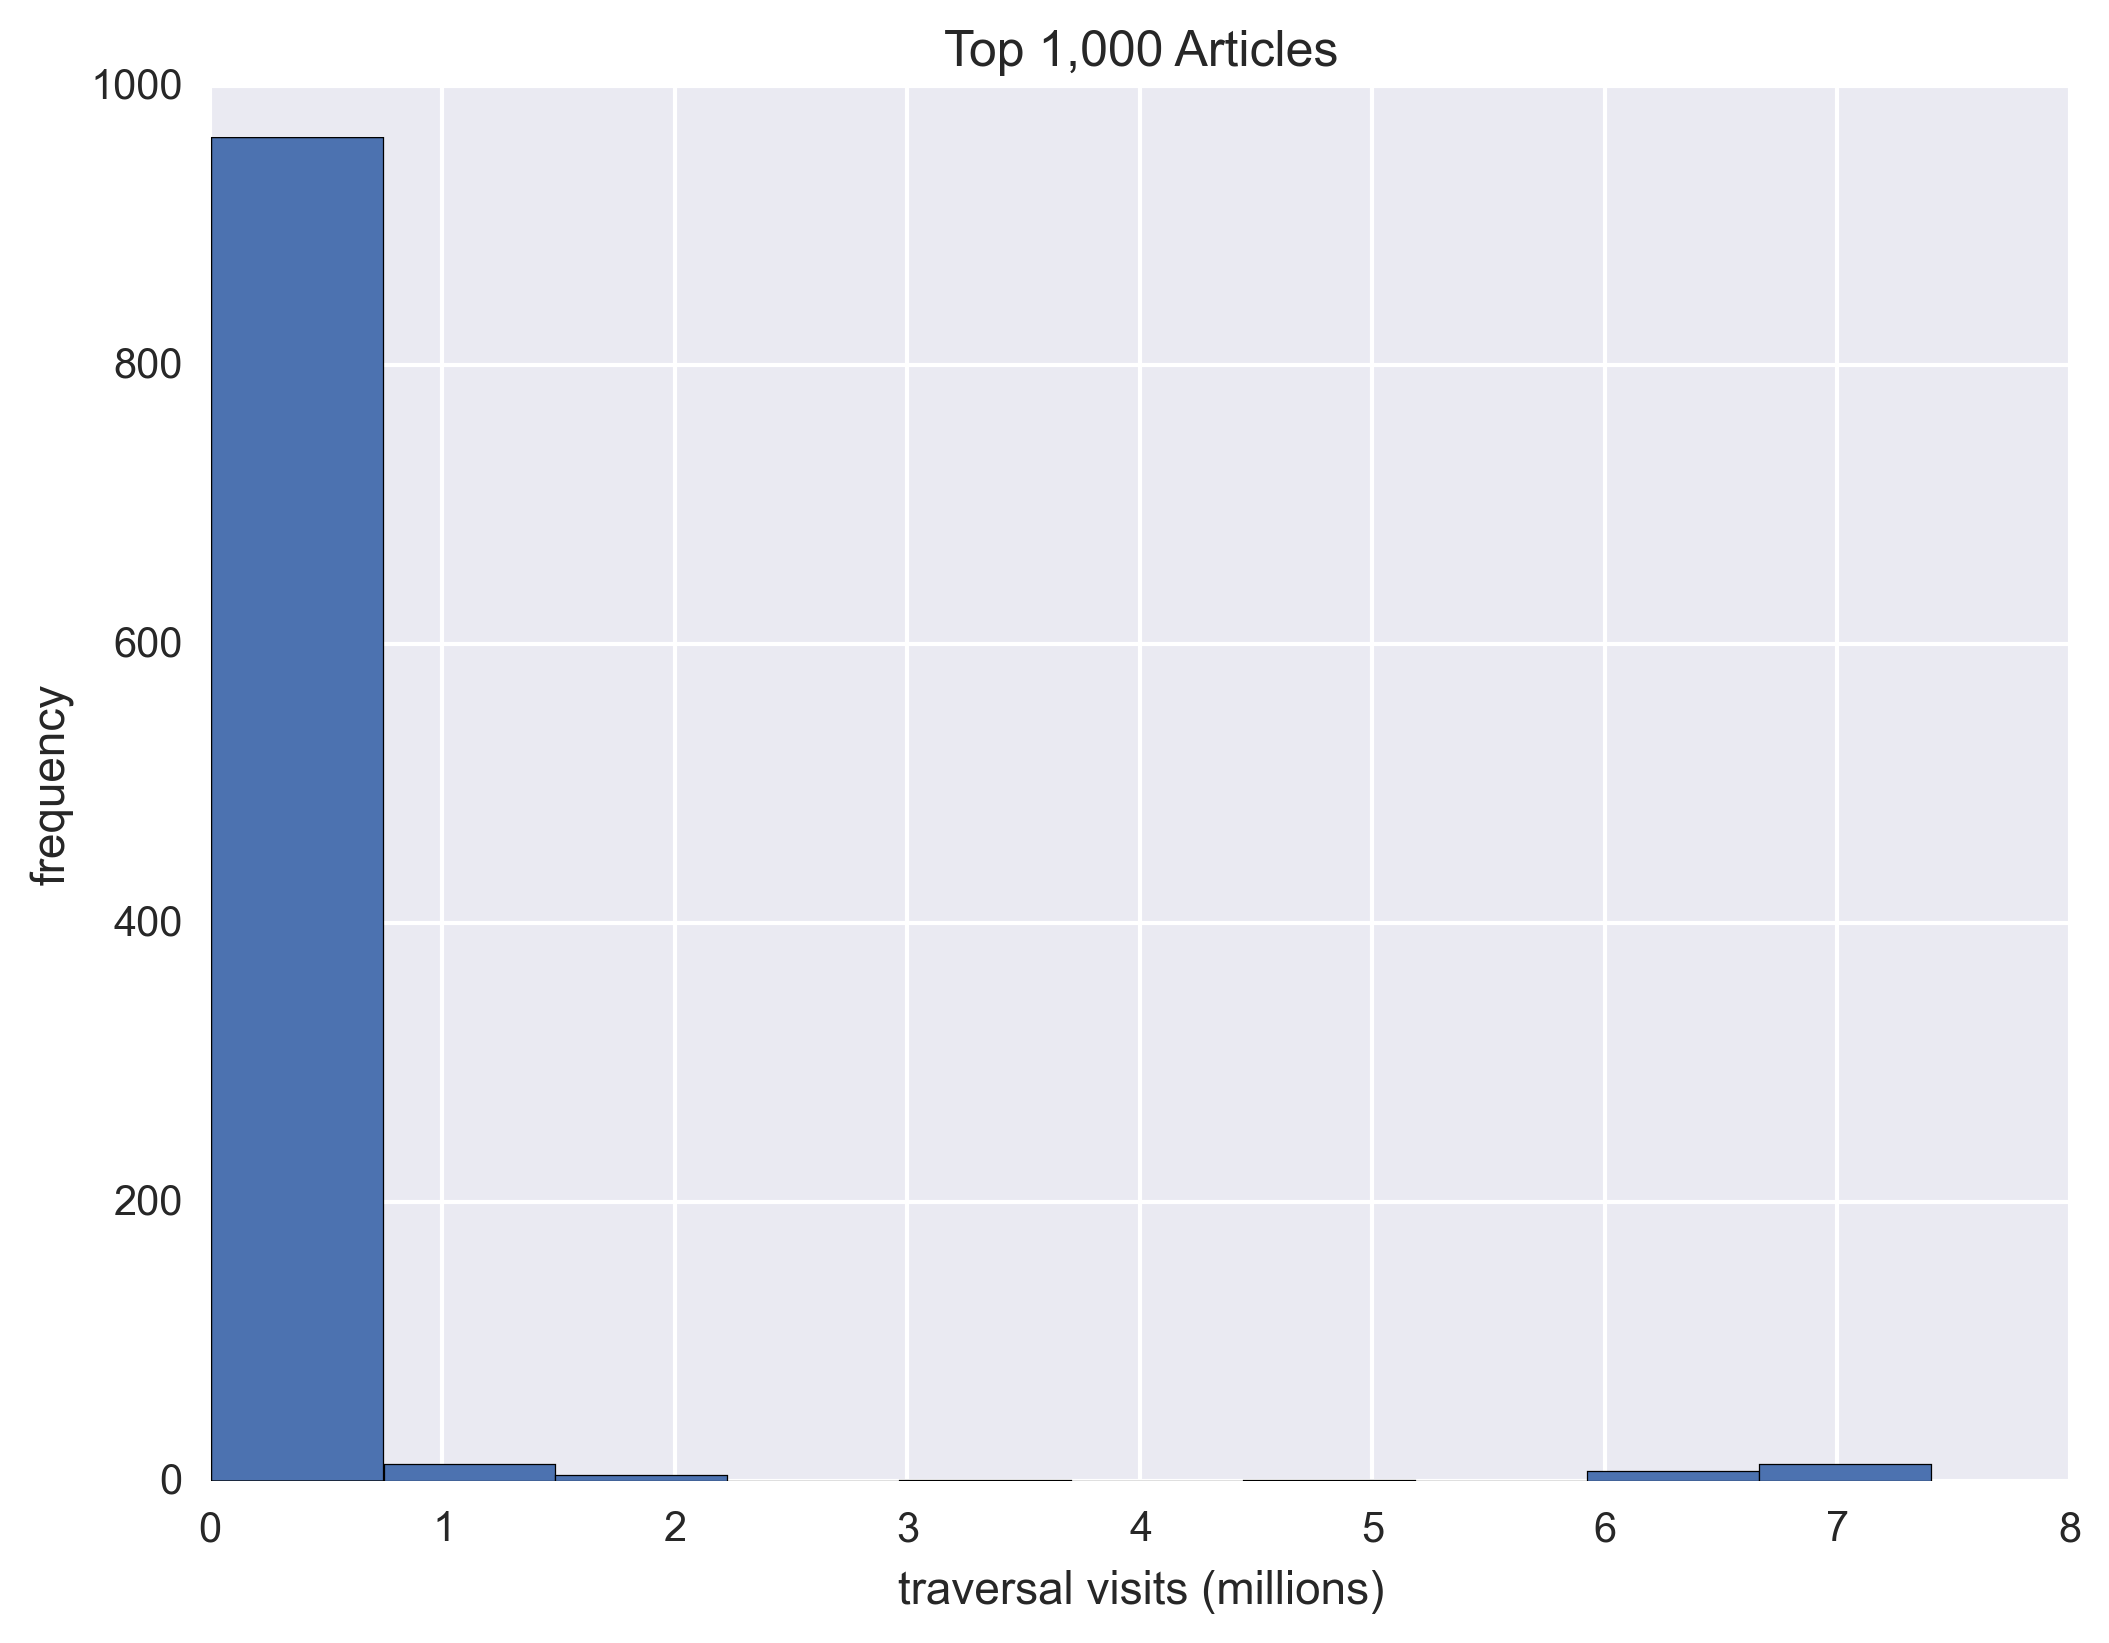
\includegraphics[width=.9\linewidth]{graphics/top_1k_article_traversals.png}
\end{subfigure}%
\begin{subfigure}{.5\textwidth}
  \centering
  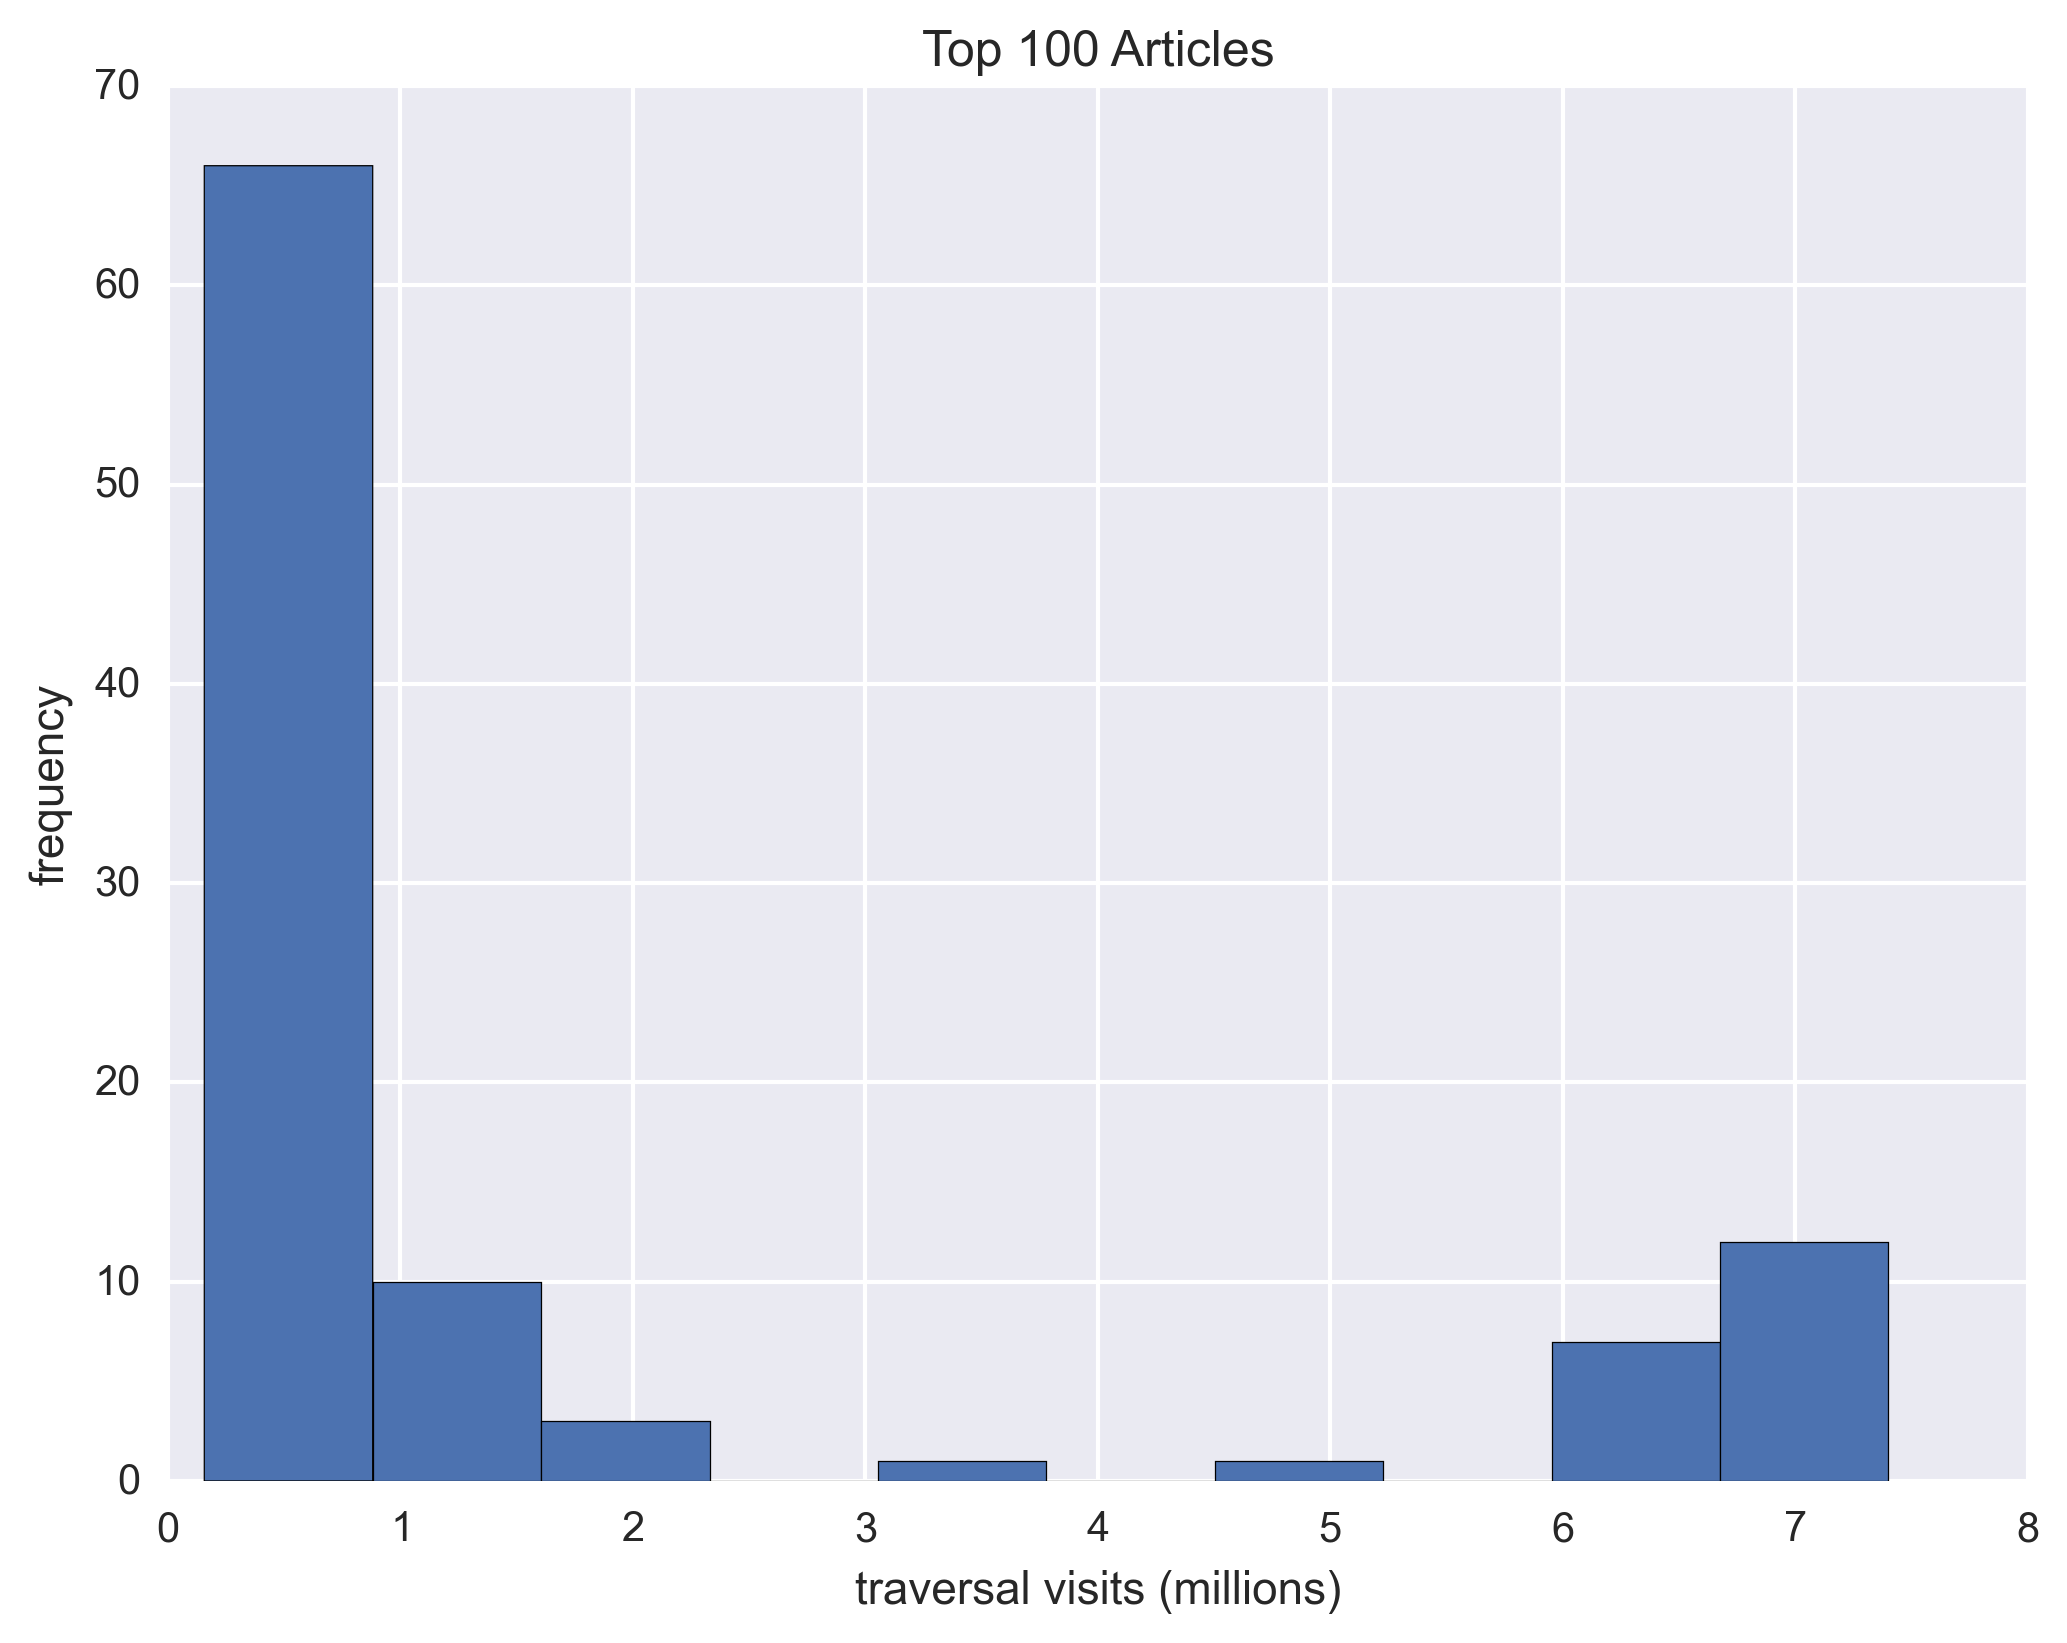
\includegraphics[width=.9\linewidth]{graphics/top_100_article_traversals.png}
\end{subfigure}
\end{figure}


The highest ranking articles include Philosophy alongside related articles such as "Existence", "Quality", and "Reality".

\begin{figure}[H]
\centering
    \caption{highest ranking articles by number of traversal visits}
        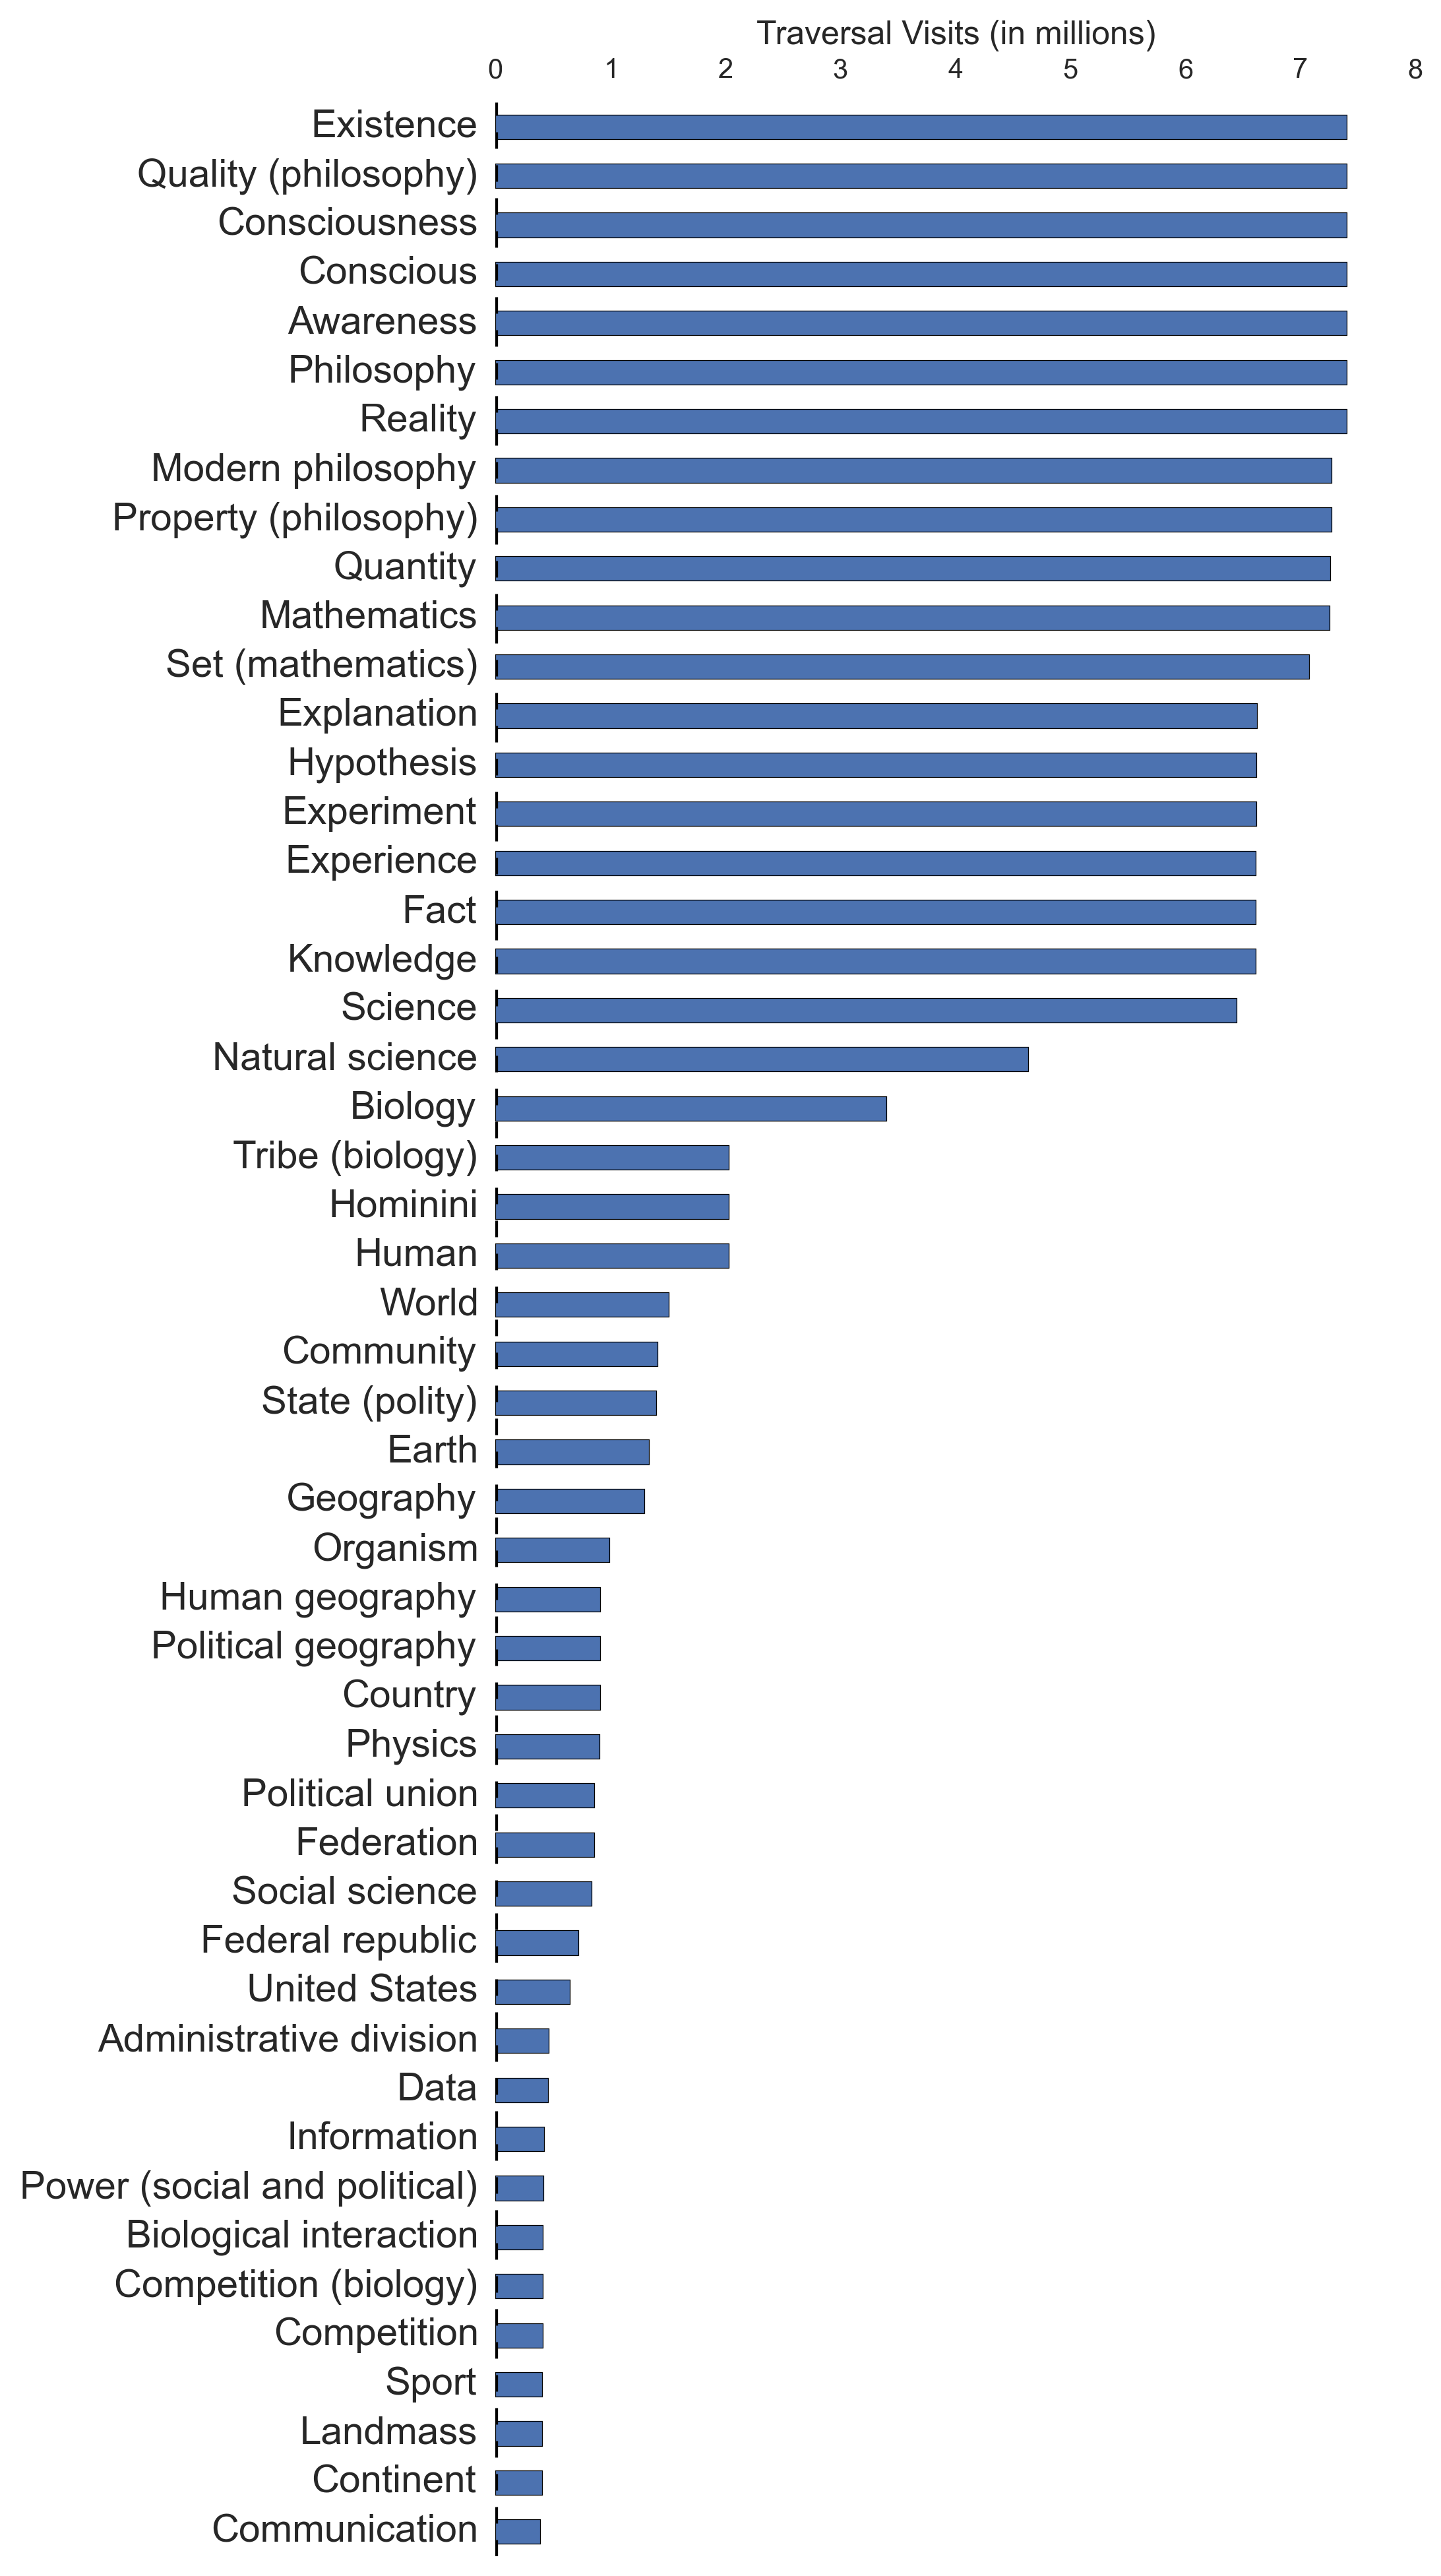
\includegraphics[width=0.6\textwidth]{graphics/articles_ranked.png}
\end{figure}


The recurrence of an exact number of traversal visits suggests some articles are part of a cycle. 
The "Philosophy" article for example sits in what seems like a cycle of seven other articles; "Hypothesis" appears to sit in a 
cycle of 6 other articles including "Experiment", "Fact", and "Knowledge".
To confirm the suggested cycle structure, we recorded the history of articles traversed along a path. 


\subsubsection{A flow from general to specific}

The highest ranking articles by traversal visits are 
broad, global topics: 
many are academic disciplines such as "Science," "Math," 
"Geography," "Biology," and "Physics"; others are abstract fundamental concepts such as 
"Community", "State", "Earth", "Information", "Communication", and "Power."
Since traversal visits measure the accumulation of First Link visits in Wikipedia, 
the highest ranking articles suggest a flow from specific to general. 
For example the flow of First Links for the "Banana" article begins at a very concrete
and specific topic then flows into progressively broader and broader disciplines, eventually 
culminating at "Philosophy: "Banana" links to the broader category of "Fruit," which then links to 
"Botany," eventually "Biology," then "Science" and ultimately "Philosophy." 

One means to measure the specificity of an article is to identify the number of synonyms available for a word or topic. The reasoning here is that a  broader topic likely has many more synonyms relative to a specific, concrete topic. Banana has fewer synonyms than botanical for example. To quantify the observed flow, we measured the number of synonyms the article title contained in WordNet---the largest lexical database of the English language. We find the highest ranking 100 articles have on average 5 more synonyms than the typical article; a difference of 2.5 synonyms if we compare the median number of synonyms in each group. As suggested by the median, many articles have no synonyms as we might expect, because titles with more than one word are not likely to appear in a thesaurus. Since many articles have no synonyms, we also compared the number of synonyms in the highest-ranking versus typical article, this time excluding all articles without at least 1 synonym. We still find the highest ranking 100 articles with an average of 9.0 (median of 7.0) synonyms whereas the remaining articles on average 5.8 synonyms (median of 7.0), even with the exclusion of all articles without any synonyms.
The quantifiable difference in synonyms corroborates the flow of links from concrete, specific articles to broader disciplines or fundamental notions.



\subsection{Network Cycles}
By tracking the articles traversed we were able to identify the cycle structures
by the reappearance of an article in our path history.
We first identified 2-cycles, meaning a pair of articles with First Link pointing to one another.
Of the 11 million articles, 84 thousand are 2-cycles. 
The highest ranking 2-cycles by traversal visits tend to be synonyms (or nearly so) rather than different, yet connected ideas:
"Health Care" and "Medical Case Management", "Broadcasting House" and "BBC", "Secondary Education" and "Secondary School".

\begin{figure}[H]
\centering
\caption{highest ranking 2-cycles}
    \begin{subfigure}[b]{0.8\textwidth}
        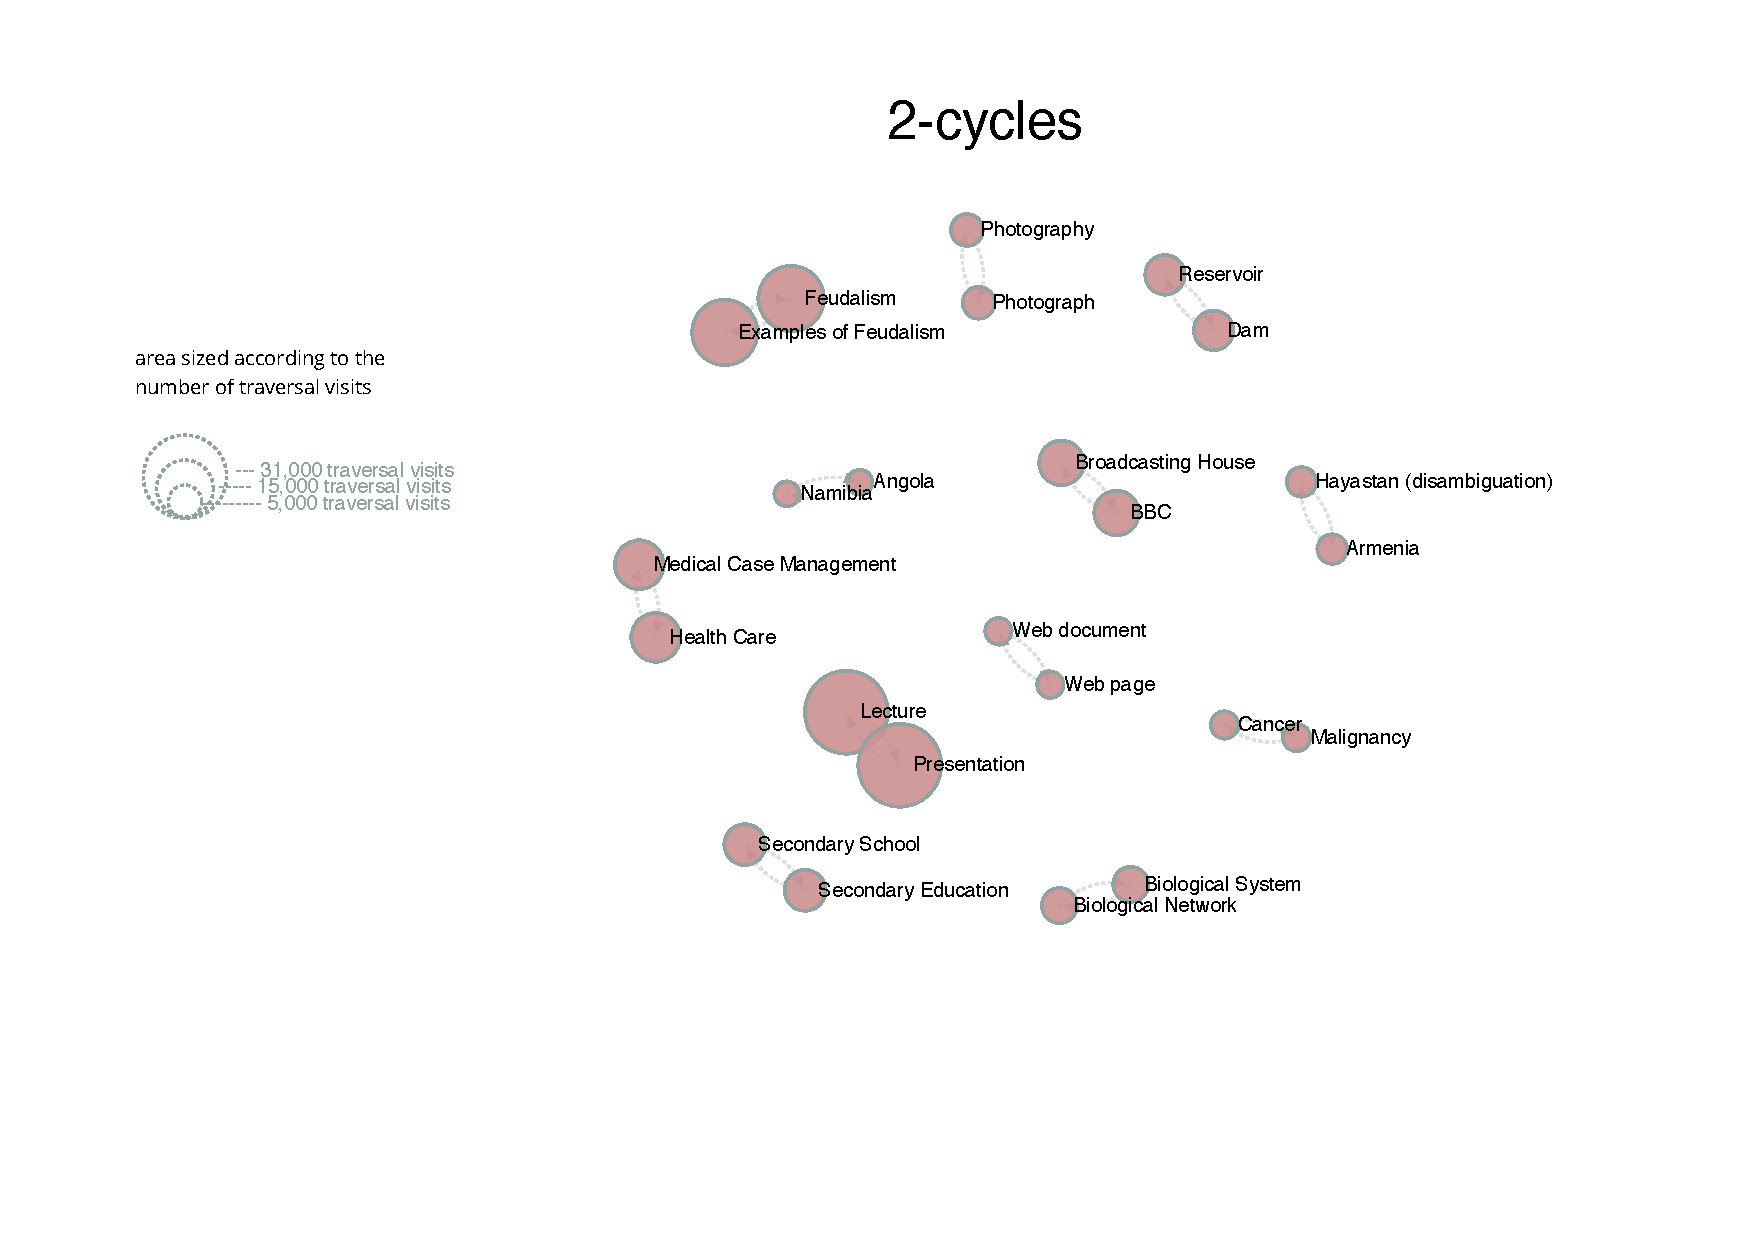
\includegraphics[width=\textwidth]{graphics/2_cycles.pdf}
    \end{subfigure}
\end{figure}



Outside of the highest ranking 2-cycles, the typical 2-cycle signals a connection between different, yet very closely related ideas. 
Link patterns such as inventor to product ("Voere" to "VEC-91"), event to organizer ("Poetry Bus Tour" to "Weave Books"), and book to author ("Anatomy of Britain" to "Anthony Sampson").

Similarly, 3-cycles captured a synonymous or close relation among 3 articles: "Tree of life (Biology)", "Tree of life (disambiguation)", 
and "Tree of life"; "Cinema of India", "Indian Cinema", and "Telugu Cinema". Once we extend our cycle size beyond a length of 6 however, 
"Philosophy" along with the remaining list of high ranking articles by traversal visits dominate.

\begin{figure}[H]
\centering
\caption{highest ranking 3-cycles}
    \begin{subfigure}[b]{0.8\textwidth}
        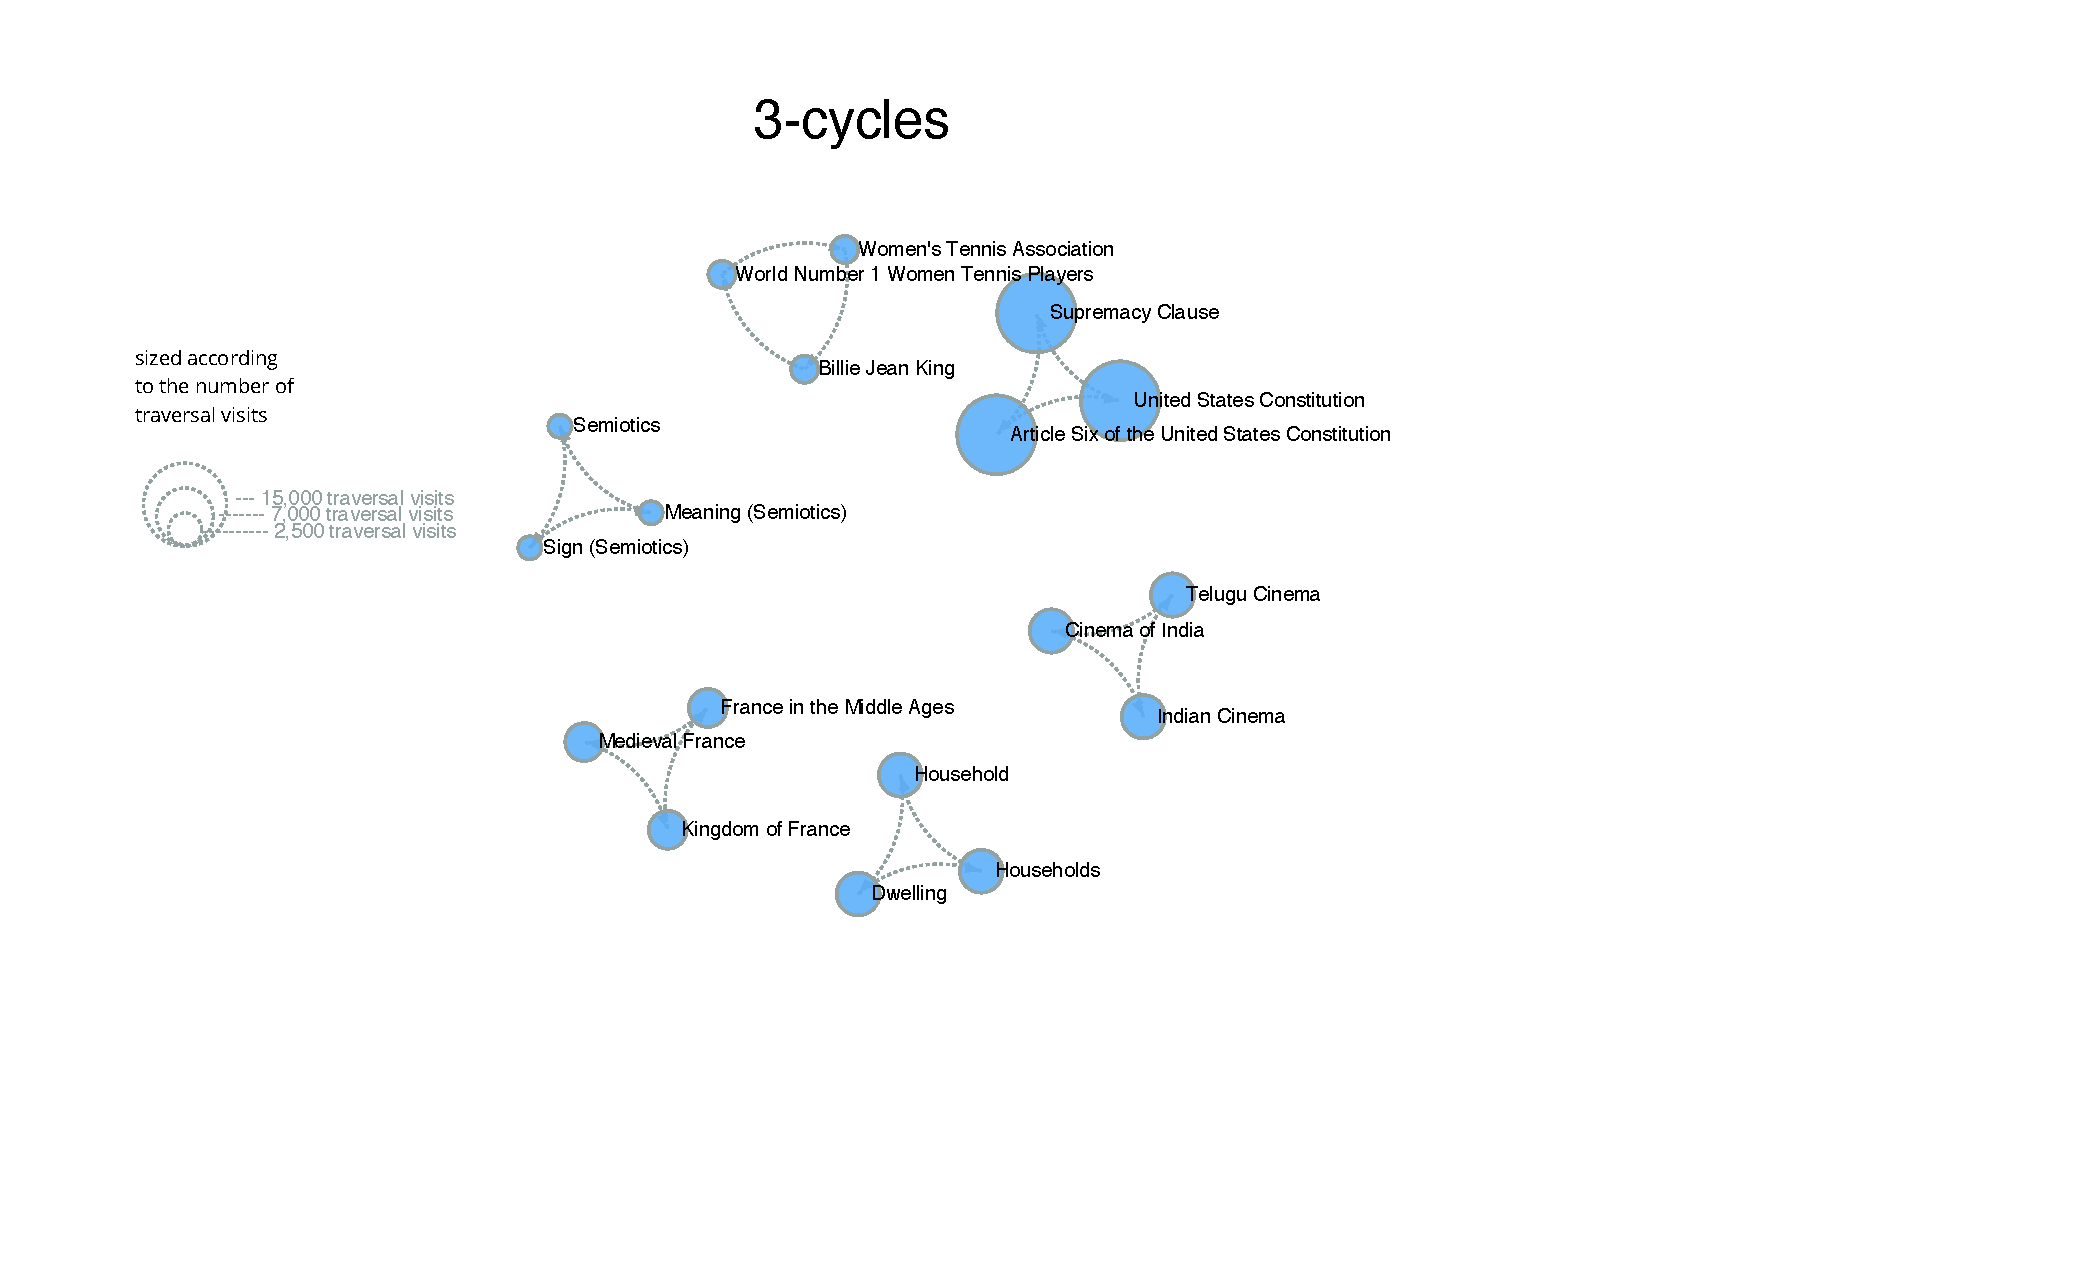
\includegraphics[width=\textwidth]{graphics/3_cycles.pdf}
    \end{subfigure}
\end{figure}

The longest cycle in the network spans 365 articles of Eastern Orthodox Liturgics for each calendar day. 
Curiously, on the last calendar day, the last article simply links back to January 1, forming a 365-cycle.
Other lengthy cycles span 60-75 articles including collections of articles on national histories such as "Japanese Eras" 
or judicial bodies such as the "Legislative Assembly of Ontario".


\subsection{Basins}
We can group articles lying on the same path to identify basins of path-connected articles, not necessarily forming a perfectly closed cycle.
Ranking basins by traversal visits, we find many of highest ranking basins are around "Philosophy" as we might expect. 
Looking beyond "Philosophy" however, we find high ranking basins around similarly foundational ideas:
"Community", "Landmass", "Federal Government", "Presentation", and "Belief System". 
These concepts naturally emerge from the First Link Network potentially indicating pillars, which 
anchor specific knowledge in a broader, simpler concept.

\begin{figure}[H]
\centering
\caption{highest ranking 3-Cycles}
    \begin{subfigure}[b]{0.8\textwidth}
        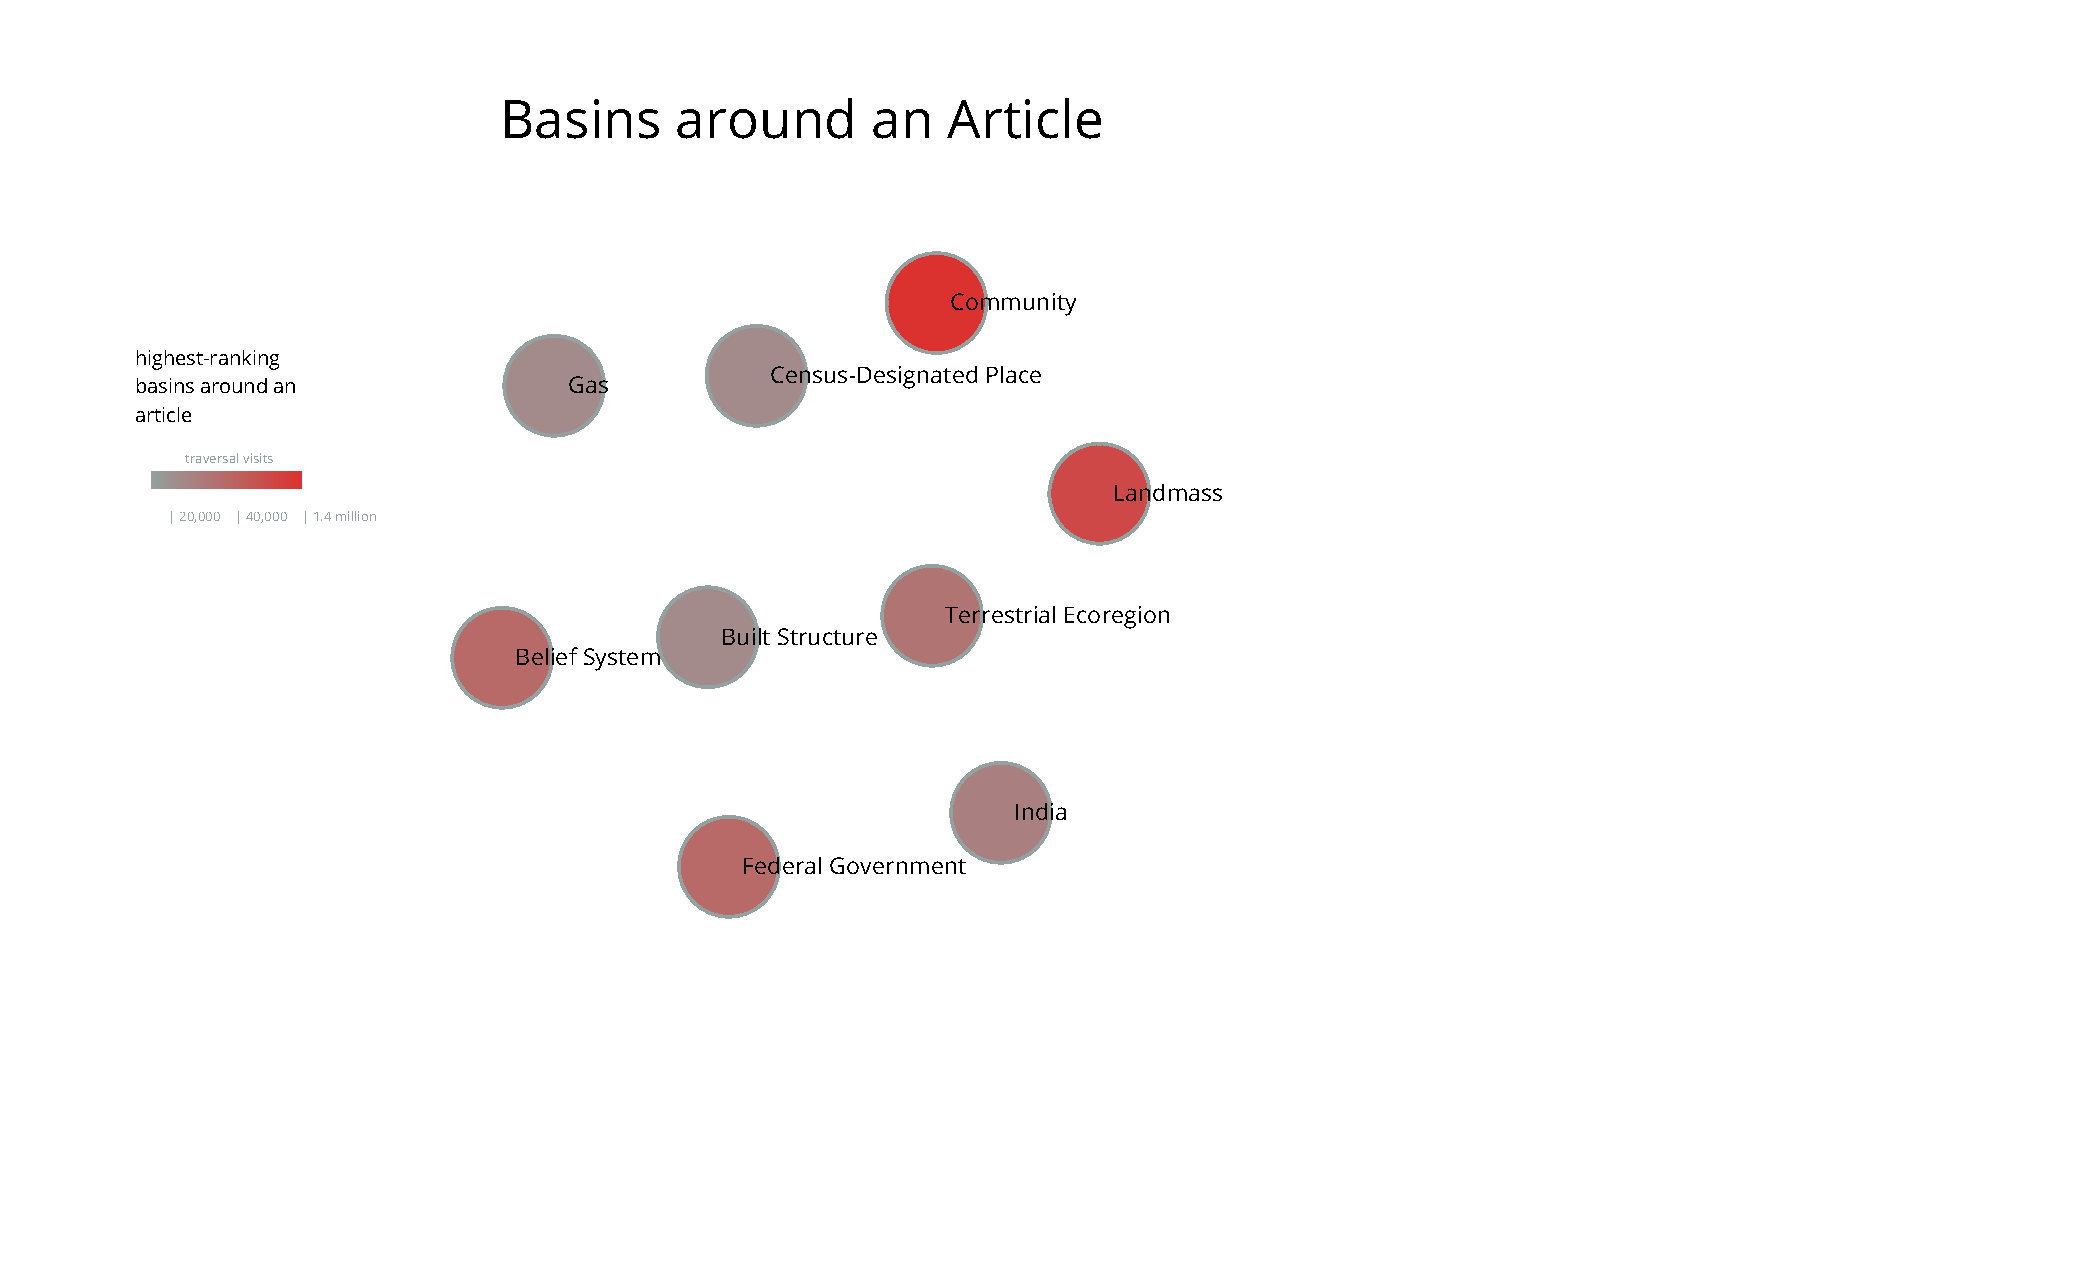
\includegraphics[width=\textwidth]{graphics/basins.pdf}
    \end{subfigure}
\end{figure}

\subsection{Path Length}

In addition to identifying cycles and cycle lengths, we also measure the traversal path length, which includes articles outside
of cycles. 
Path length measures the number of links traversed until a repeated or invalid link. 
We discovered the longest path length is also 365, matching the longest cycle of Orthodox Liturgics. 
We also found similarly lengthy paths following the evolution of a place or topic through time: 
"1953 in Scotland" or "1560s Architecture", with articles sequentially proceeding by year, decade or era.

Of the 11 million articles, 5.5 million had an invalid link or linked back to the same article, yielding a path length of zero. 
The most common path length is 29, with an interquartile range (26, 30).
The distribution of path lengths is similarly scale-free with few articles at the extreme of 365 path lengths, while the majority 
is between 26-30: 

\begin{figure}[H]
\centering
    \caption{Path Length Distribution}
    \begin{subfigure}[b]{0.5\textwidth}
        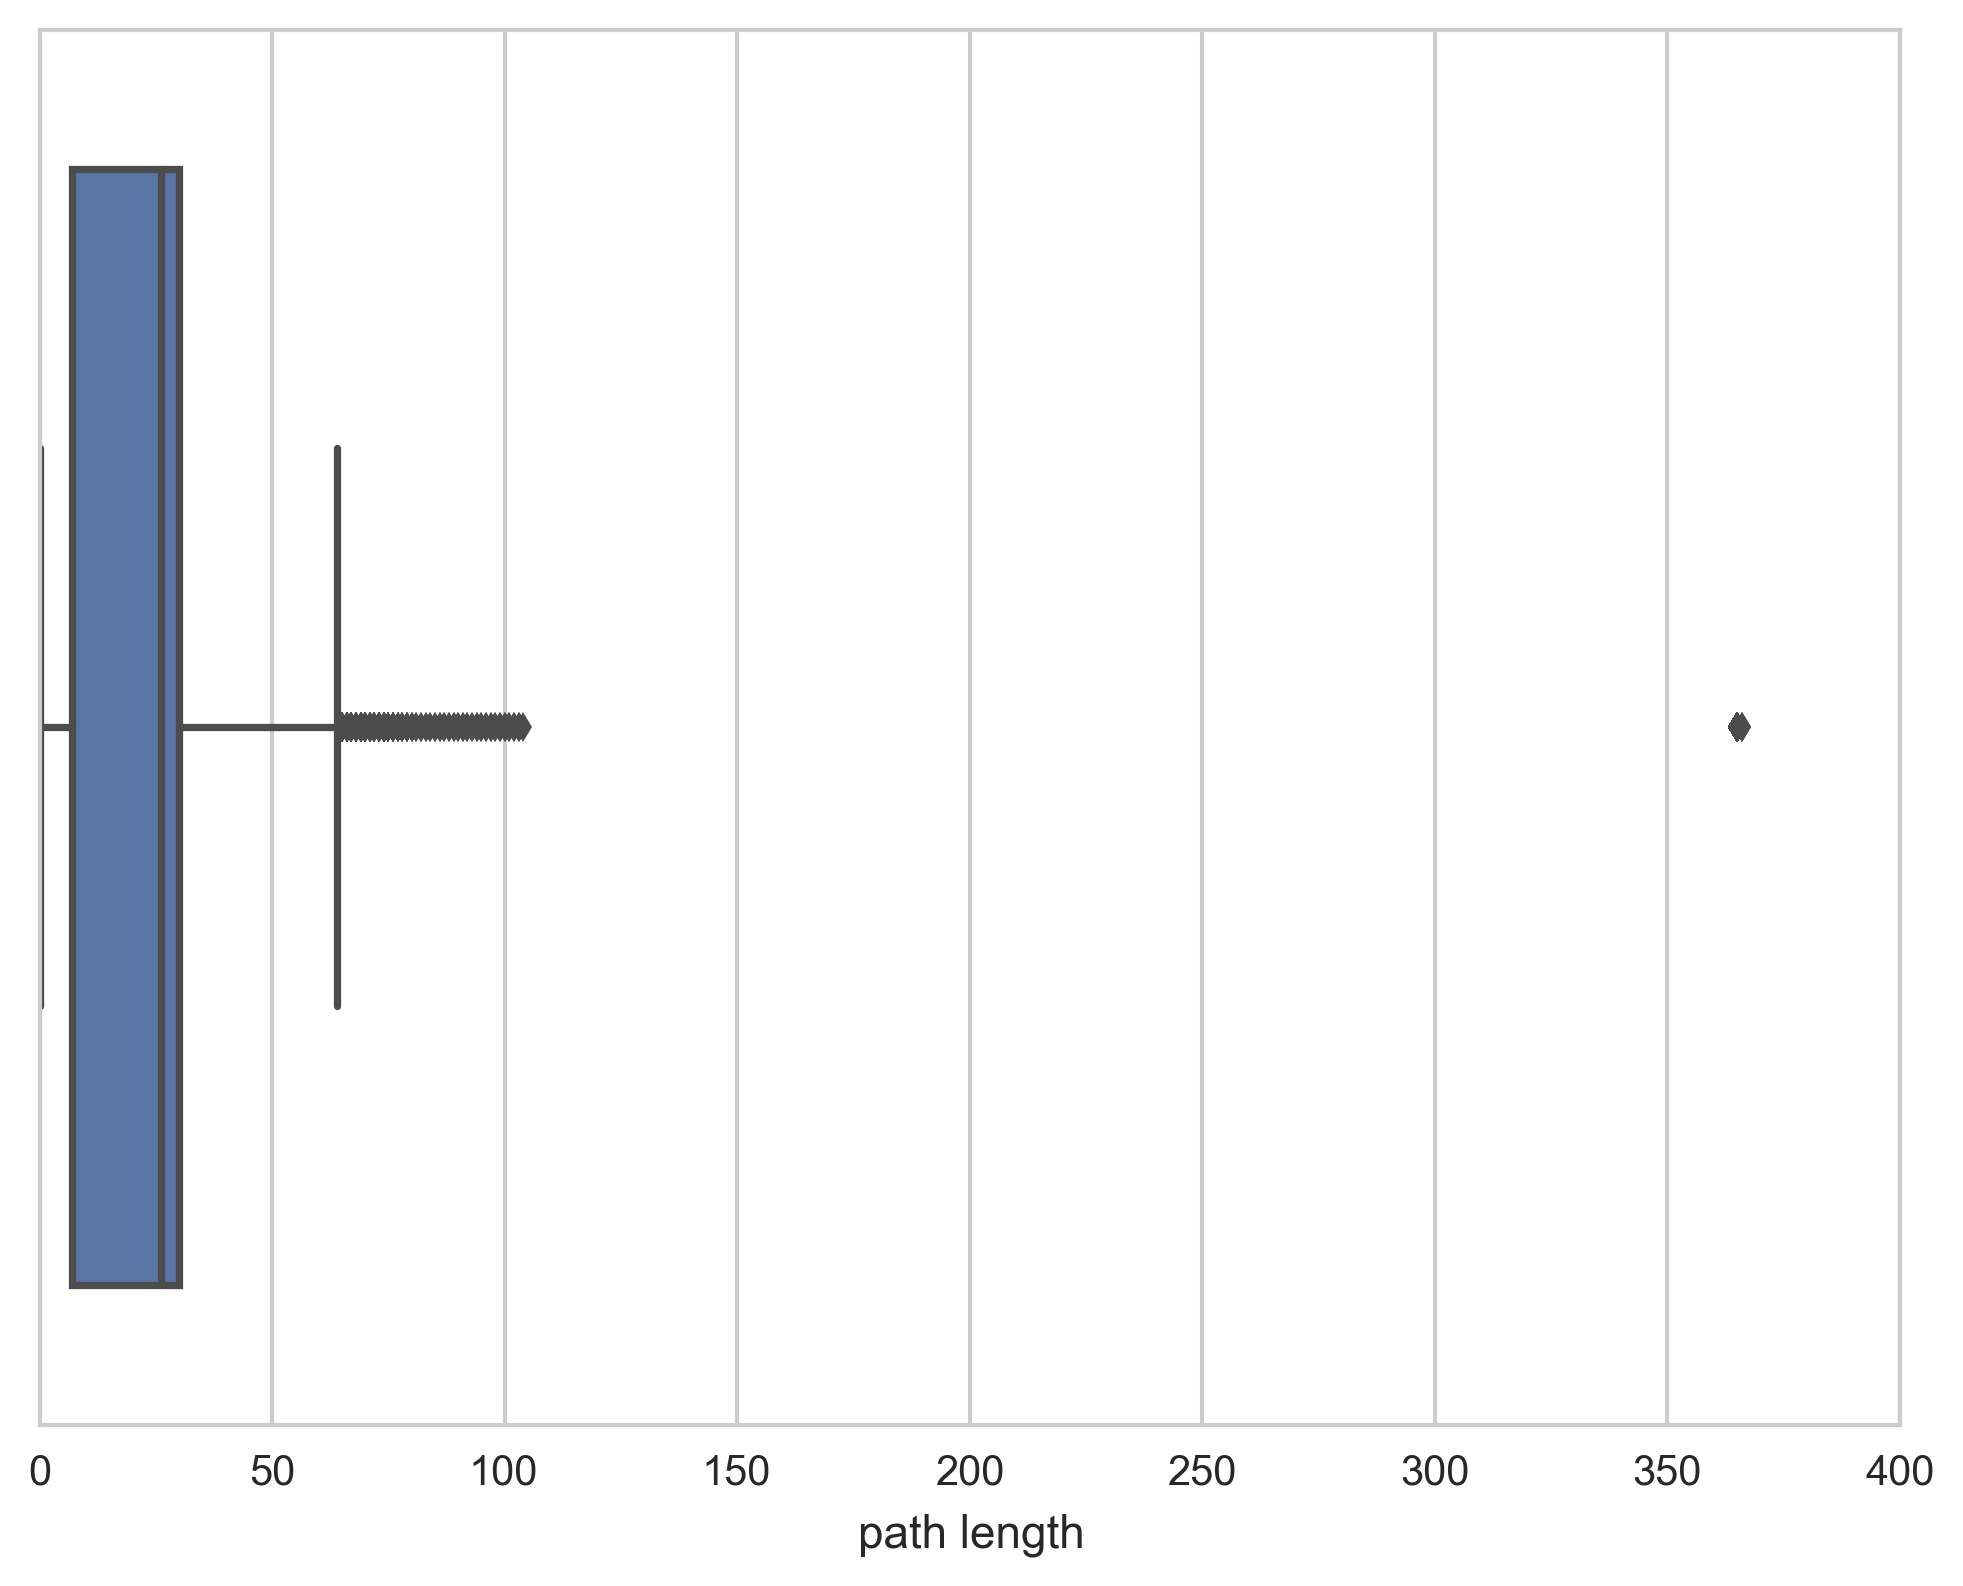
\includegraphics[width=\textwidth]{graphics/path_lengths_boxplot.png}
    \end{subfigure}
\end{figure}
\begin{figure}[H]
\centering
    \caption{Longest Path Lengths}
    \begin{subfigure}[b]{0.5\textwidth}
        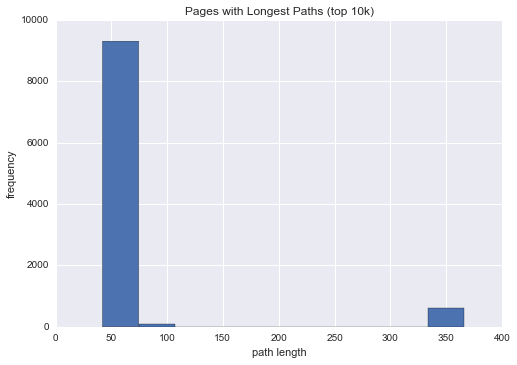
\includegraphics[width=\textwidth]{graphics/top_1k_path_length.png}
    \end{subfigure}
\end{figure}


\subsection{Traversal Funnels}

Measuring only traversal visits however is limiting as it does not distinguish whether a particular article in a cycle 
is a funnel, directing many more paths inside the cycle than others. 
To distinguish among articles in a cycle, we also measured traversal funnels, or the number of 
paths an article directs towards a cycle. Here we count the number of traversal visits up to a cycle, 
so that accumulation does not flow to all articles in a cycle.
The importance here is to distinguish an article that happens to be connected to another article with many traversal visits 
from an article directly funneling many paths.

Measuring traversal funnels reveals a dramatically different structure where "Philosophy" stands unmatched by orders of magnitude:

\begin{figure}[H]
\centering
    \caption{Top Funnels}
    \begin{subfigure}[b]{0.9\textwidth}
        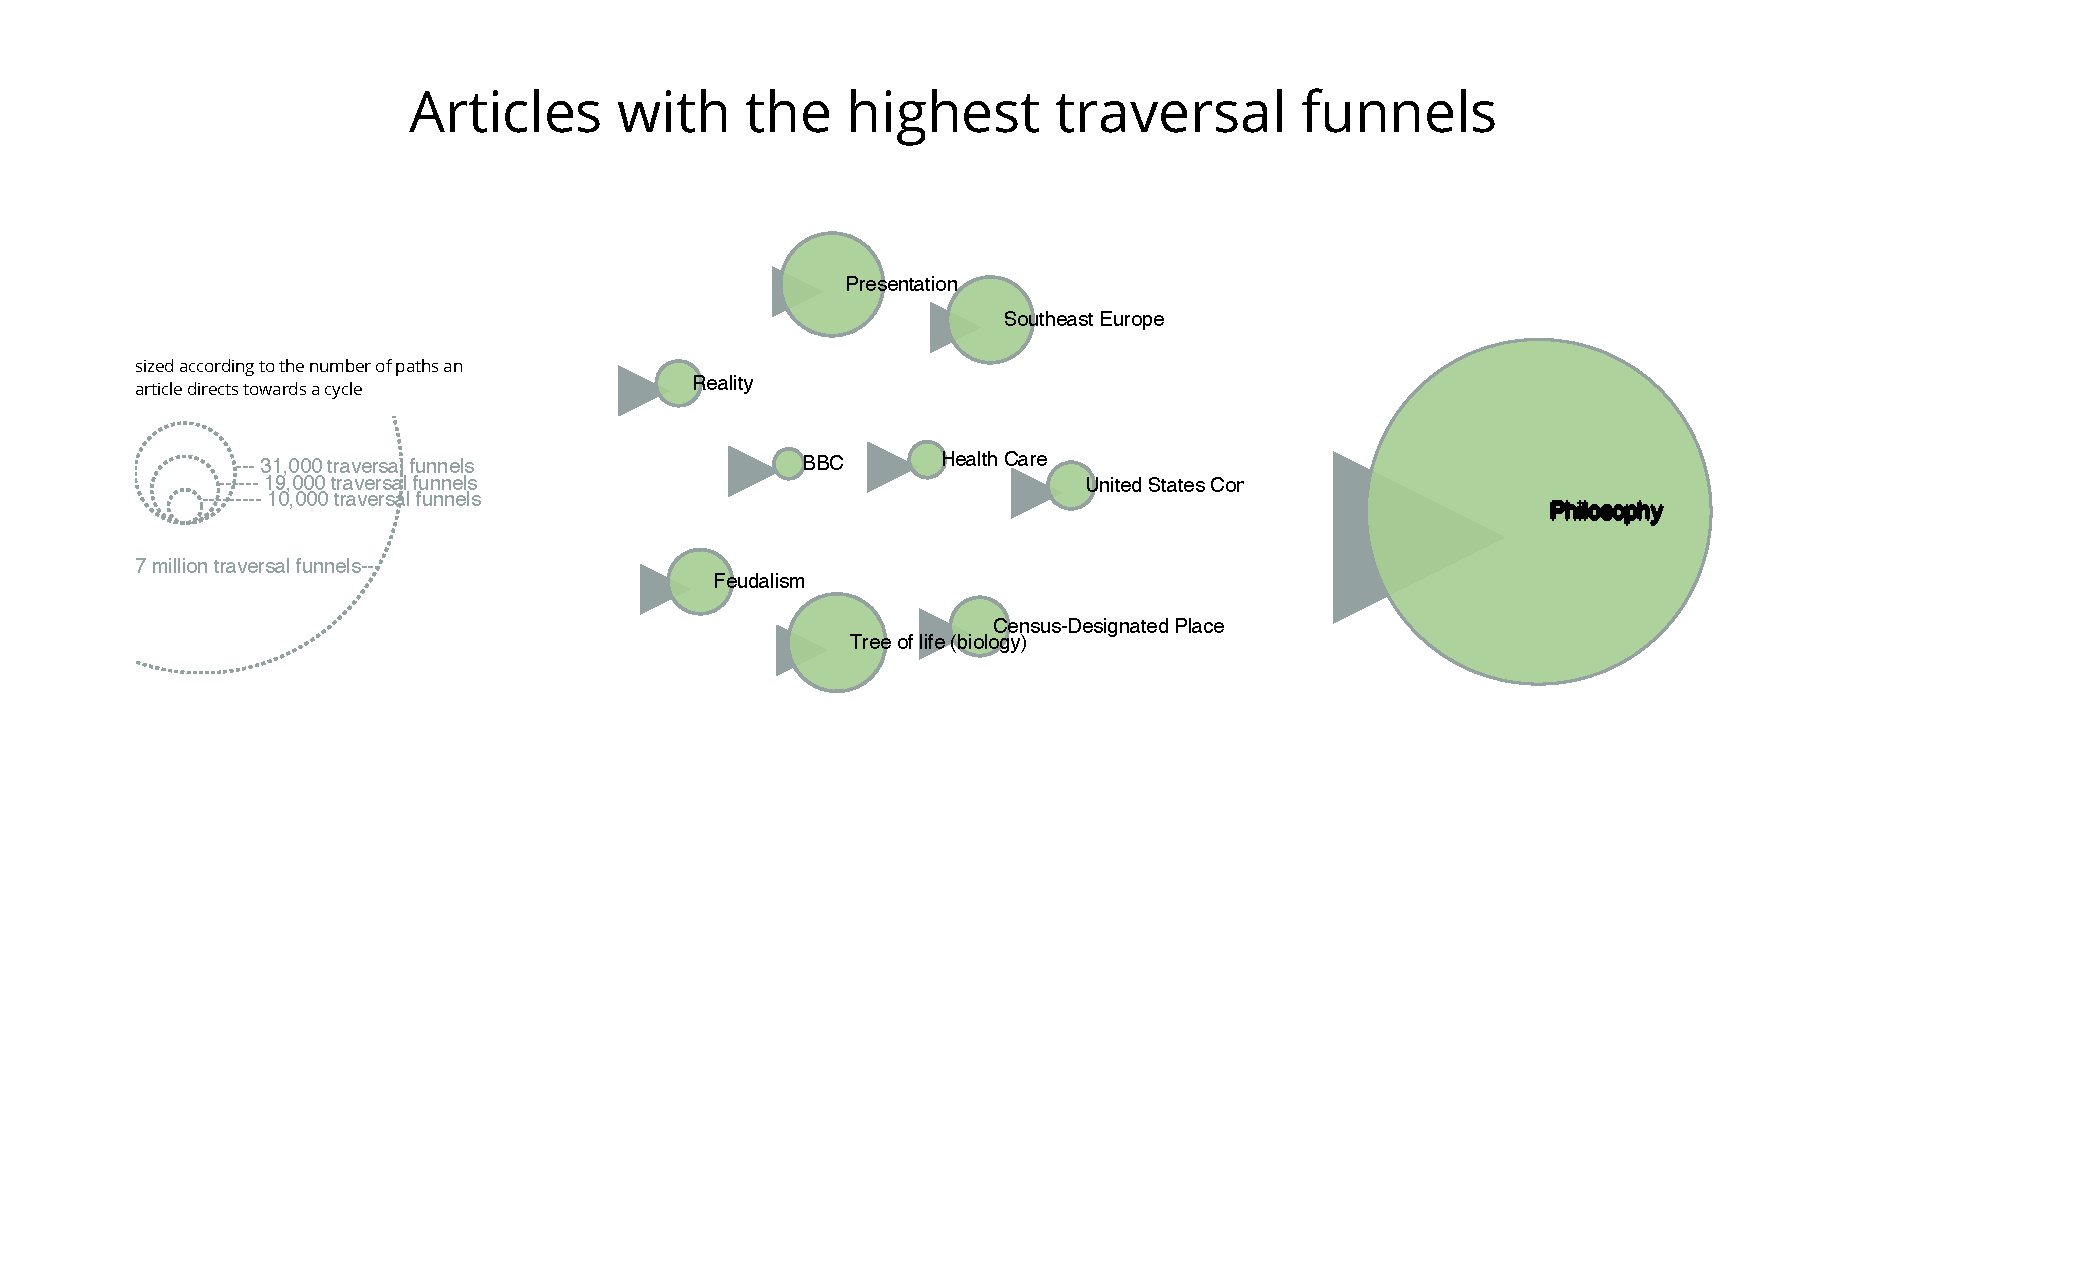
\includegraphics[width=\textwidth]{graphics/funnels.pdf}
    \end{subfigure}
\end{figure}

Philosophy is not only a stand out the number of traversal visits, but also by the number articles "Philosophy" funnels into
its cycle. Of any article, the number of traversal funnels Philosophy holds exceeds 
all others by at least two orders of magnitude.
Next to the contribution of the largest funnels, "Philosophy" is a singularity. 
In proportion, "Presentation" holds only $0.4\%$ next to the number of traversal feeds for "Philosophy".
The second contributor to the Philosophy cycle is "Reality", funneling in a mere $.2\%$ of traversals visits in the cycle.
Nevertheless, the other high ranking funnels are remarkably topical, culturally and politically important ideas.  For example, "Health Care", a recently high-contested legislative topic appears high on the list---Google trends indicates an uncharacteristic spike in search frequency between August-2009 and February-2010.
Other high ranking articles include key historical events such as the "Cold War" or critical scarce resource with recent 
media discussion such as "Fossil Fuel".
This coincidence of recent relevance and traversal feed rank suggests the First Link Network measurably represents
meaningful relationships not only among ideas, but also to English-speaking society. 


%========================Conclusion====================================
\section{Reflections}

The findings here should only be considered within the limitations of their context.
We examined only the English version of Wikipedia at a particular moment in time.
Furthermore, we only studied the First Link in the main body of each article
as a means to related one article to another. Finally, Wikipedia, while the largest 
collection of human knowledge, is rife with the biases of the many contributing editors ((cite))
. Nevertheless, the findings do reveal
generalizable relationships, point to foundational notions, and uncover many curiosities.


Among the curiosities is the multiple appearance of scale-free distributions within the network. 
The three metrics we developed: path length, traversal visits, and traversal funnels are all marked 
by scale-free distributions. Few articles have most traversal visits, few paths have an exceptionally long path length, and even fewer
articles are responsible for funneling most paths. When measured against the traversal funnels, 
"Philosophy" emerges as an exceptional article by orders of magnitude. 
Nevertheless, many other foundational ideas emerged naturally within the First Link Network. 
Basins around "Community", "State", and "Science" reveal a foundational structure within the network. 
More curious is the emergence of recently prominent political and economics topics such as "Fossil Fuel" and "Health Care" 
within the highest ranking funnels. 
Wikipedia seems to reflect not only timeless foundations, but also the topical (at least within English speaking society).

Future work could analyze other language versions of Wikipedia for potentially telling cultural or regional differences as well as expand the network beyond the First Link to a subset or potentially all links.
These findings also form the basis for the creation of a taxonomy where 
every idea, event, or object sits within a hierarchy of connected notions.
The taxonomy would extend a traditional word thesaurus beyond mere synonyms to a related hierarchy of concepts.
Applications could range from an enhanced thesaurus of ideas to psychological insights into how humans form associations.
Specifically, an ever-evolving reference of related hierarchical concepts can be applied to search engine algorithms 
or natural language processing.



\blfootnote{
- thank you to my friend RJ for pointing out the xkcdc comic about links to Philosophy
}


\newpage 

\section{Supplementary}

\begin{figure}[H]
\centering
\caption{highest ranking 2-Cycles}
    \begin{subfigure}[b]{0.8\textwidth}
        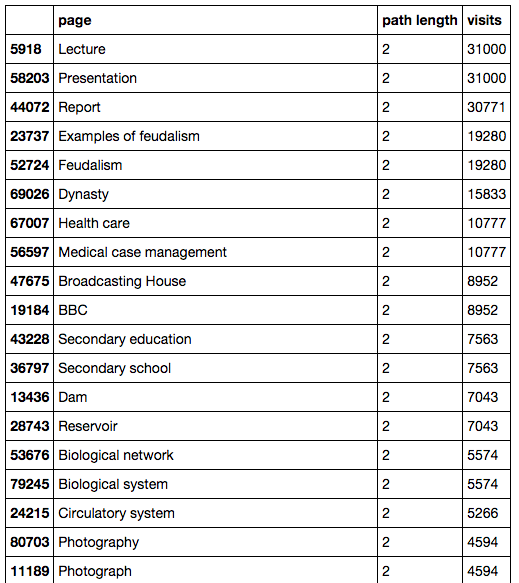
\includegraphics[width=\textwidth]{graphics/top_2loops.png}
    \end{subfigure}
\end{figure}

\begin{figure}[H]
\centering
\caption{highest ranking 2-Cycles}
    \begin{subfigure}[b]{0.8\textwidth}
        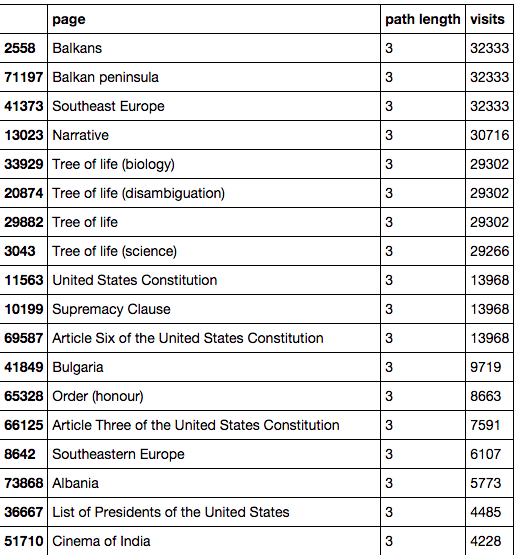
\includegraphics[width=\textwidth]{graphics/top_3loops.png}
    \end{subfigure}
\end{figure}
\begin{figure}[H]
\centering
    \caption{Top Funnels}
    \begin{subfigure}[b]{0.5\textwidth}
        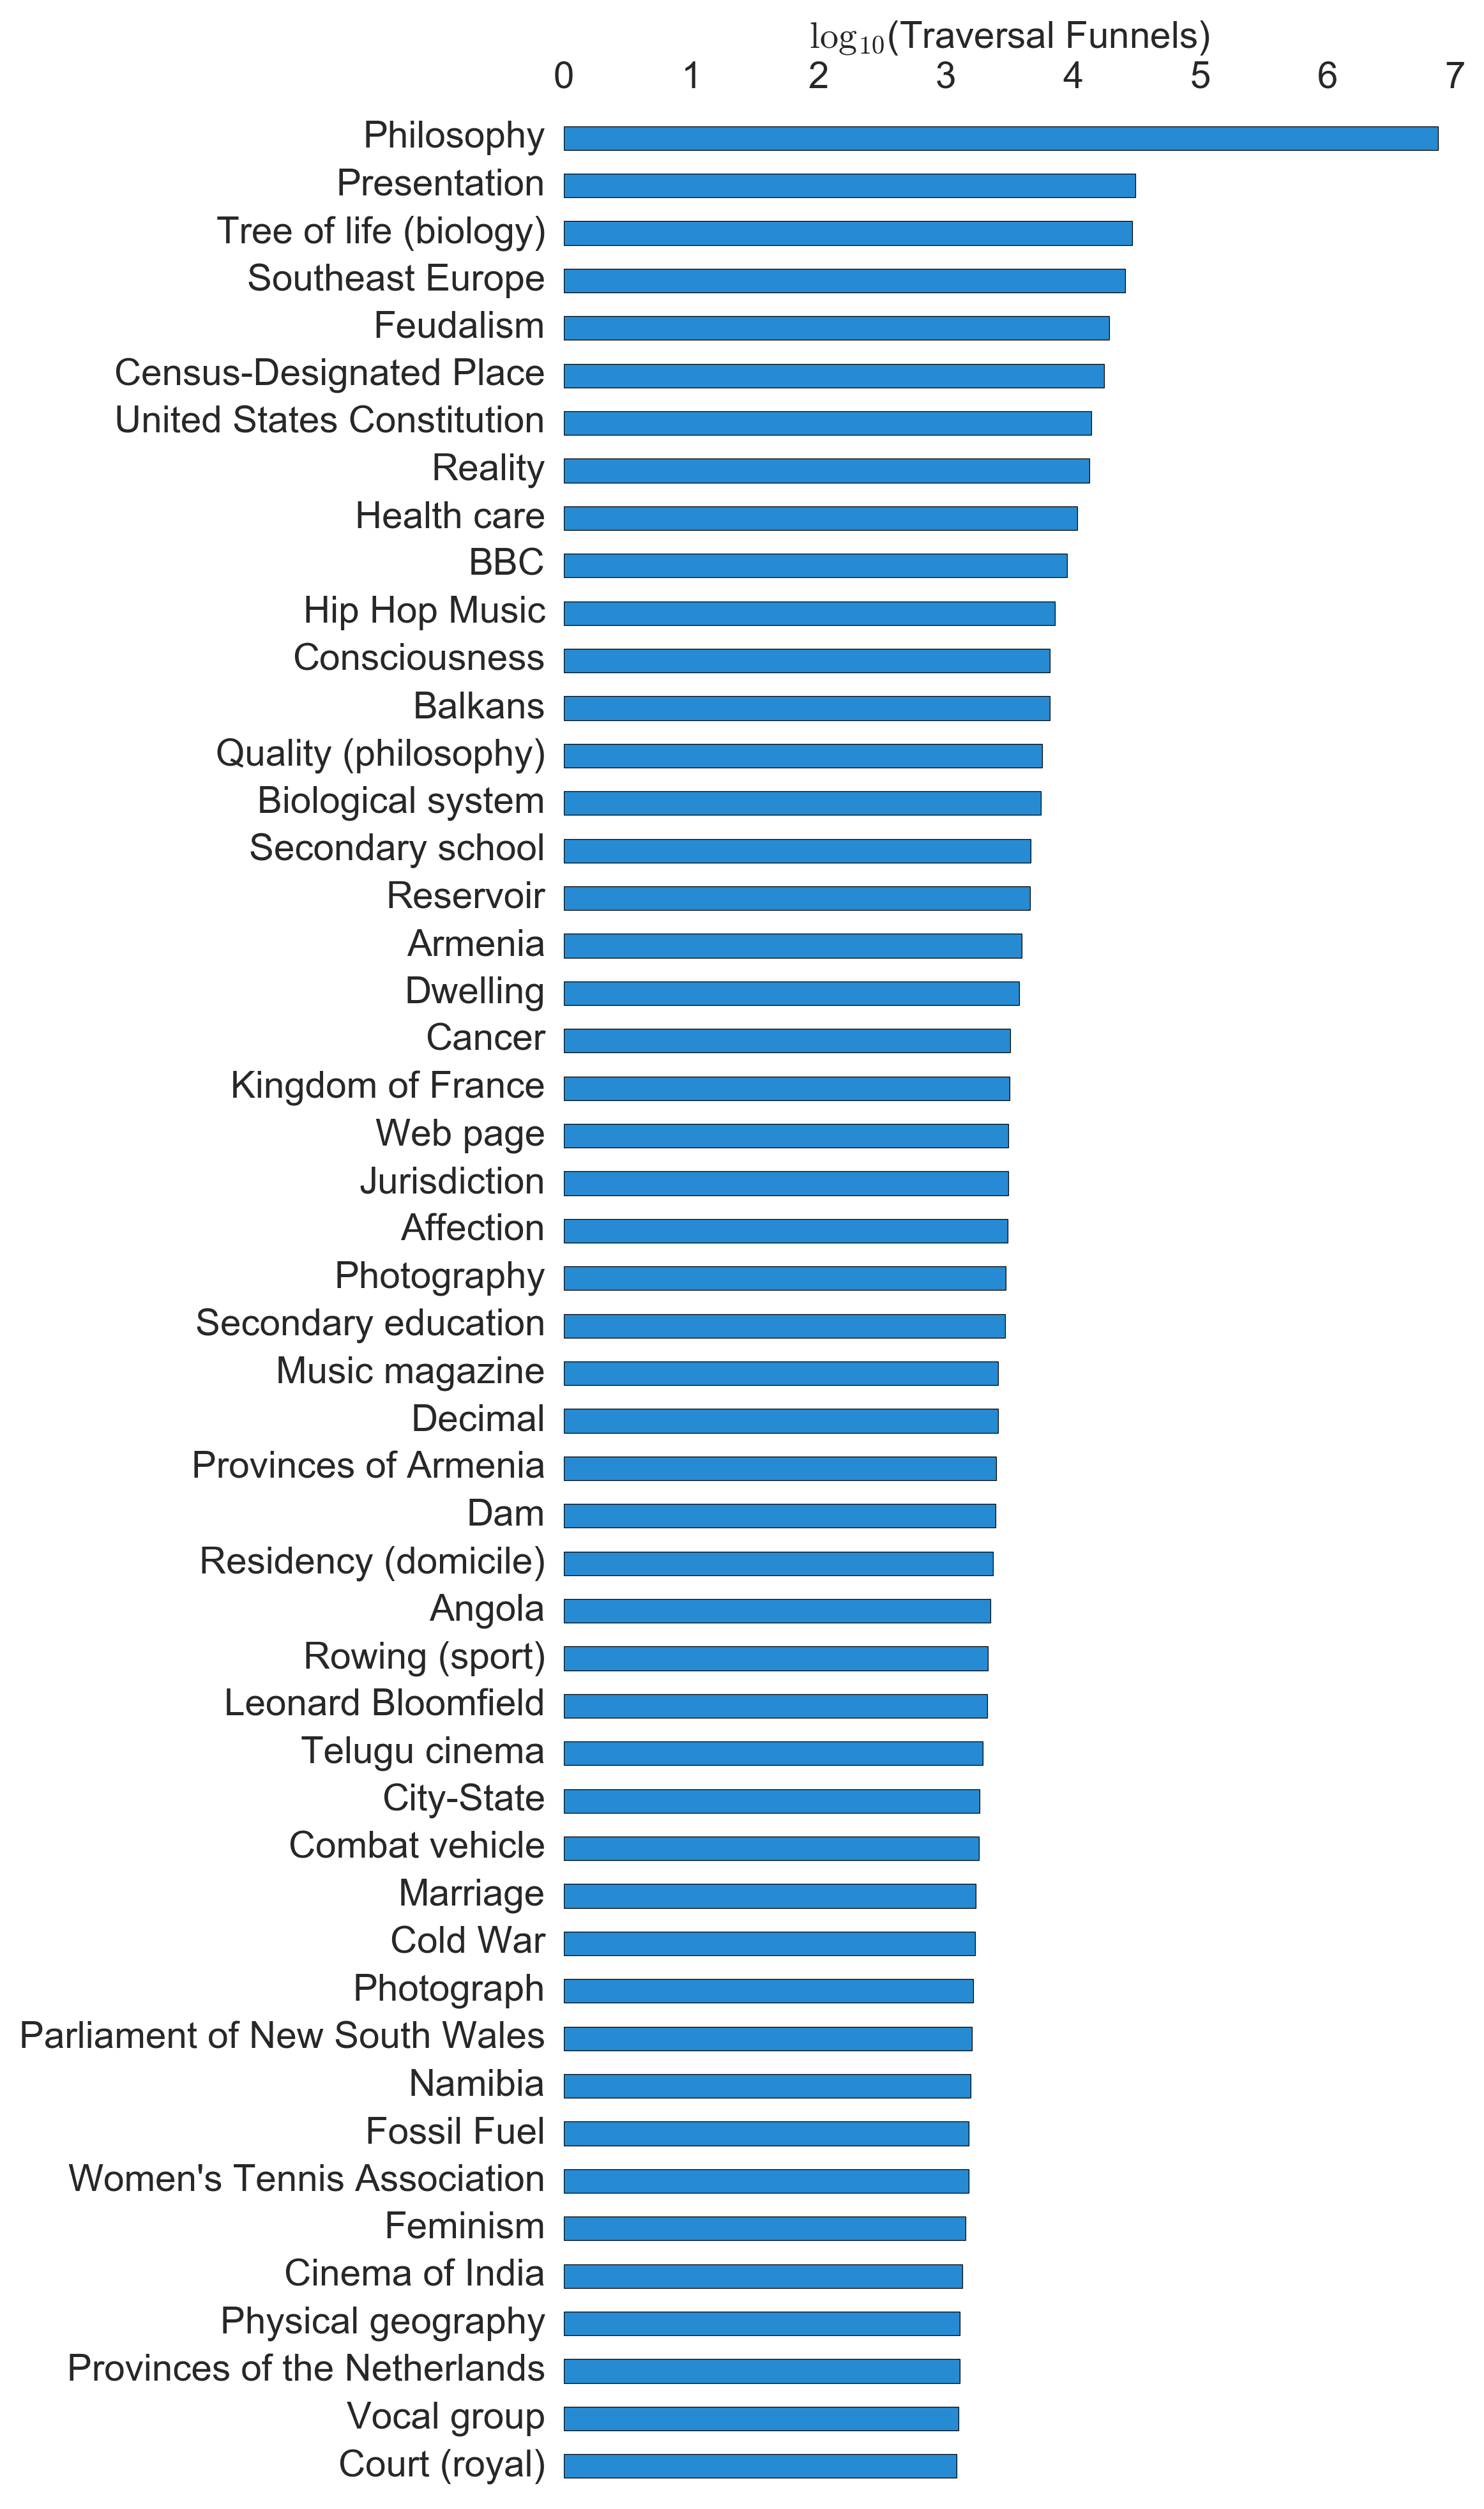
\includegraphics[width=\textwidth]{graphics/top_funnels.png}
    \end{subfigure}
\end{figure}
%========================Style Guide====================================


%\newpage
%
%\section*{Style Guide}
%
%\begin{itemize}
%\item Web Terms
%    \begin{itemize}
%        \item \bt{article} instead of page
%        \item \bt{invalid link} (instead of dead or bad link)
%    \end{itemize}
%\item Measurements
%    \begin{itemize}
%        \item \bt{traversals visits} = node weight based on number of paths crossing an article.
%        \item \bt{path length} = number of articles traversed until an invalid link or a repeated article
%        \item \bt{traversal funnels} = traversals before a cycle is reached.
%    \end{itemize}
%\item Network Properties
%    \begin{itemize}
%        \item \bt{cycle} = permutation or a true loop
%        \item \bt{path-connected articles} for both cycles and articles along the same path leading to an 
%    invalid link
%        \item \bt{basin} a path-connected group of articles (not necessarily forming a cycle)
%    \end{itemize}
%\end{itemize}
%
%- add quotes around article names: Philosophy should be "Philosophy"
%
%- add thank you to RJ for pointing out the Blog Post


\end{document}
